% ======================
% Bachelor Thesis LaTeX
% fixed version 2025‑04‑30
% ======================
\documentclass[a4paper,12pt]{article}

% ---------- Geometry / Layout ----------
\usepackage[margin=2.5cm]{geometry}
\usepackage{setspace}
\usepackage{parskip}

% ---------- Fonts ----------
\usepackage{helvet}      % default sans‑serif
\usepackage{fontspec}    % requires XeLaTeX/LuaLaTeX
\setmainfont{AUPassata_Rg.ttf}
\renewcommand{\familydefault}{\sfdefault}

% ---------- Graphics / Floats ----------
\usepackage{graphicx}
\usepackage{svg}
\usepackage{float}       % enables [H] placement
\usepackage{caption}
\usepackage{animate}
\usepackage{tabularx}   % flexible-width columns
% ---------- Mathematics ----------
\usepackage{amsmath, amssymb}

% ---------- Tables ----------
\usepackage{booktabs}    % \toprule etc.
\usepackage{pdflscape}


% ---------- Lists / Enumeration ----------
\usepackage{enumitem}

% ---------- Code Listings ----------
\usepackage{listings}
\lstset{
  language=Python,
  basicstyle=\ttfamily\footnotesize,
  keywordstyle=\color{blue},
  stringstyle=\color{red},
  commentstyle=\color{gray},
  backgroundcolor=\color{gray!10},
  frame=single,
  breaklines=true,
  showstringspaces=false,
  captionpos=b,
  tabsize=4
}

% ---------- Hyperlinks & TOC ----------
\usepackage{hyperref}
\usepackage{tocloft}

% ---------- Bibliography ----------
\usepackage{natbib}

% ---------- Colours ----------
\usepackage{xcolor}

% ---------- Page style ----------
\pagestyle{empty} % cover page has no numbers

% =====================================================
%                       DOCUMENT
% =====================================================
\begin{document}

% -------------------- Cover Page --------------------
\begin{center}
    % Tight top margin
    \vspace*{0.5cm}

    % Top logo
    
\includegraphics[width=0.35\textwidth]{bss_logo.png}

    \vspace{1.5cm}

    % Title
    {\LARGE\textbf{Economic Entropy and the Energetic Foundations of the Anthropocene\\[0.4em]}}

    \vspace{1em}
    {\large Bachelor Thesis}

    \vspace{1.8cm}
    {\Large Balázs Kocsis\\[0.3em]Bent Jesper Christensen}

    \vspace{2.2cm}
    
\includegraphics[width=0.20\textwidth]{university_logo.png}

    \vspace{2.2cm}
    \normalsize
    Aarhus BSS\\Aarhus University\\Department of Economics\\2025 Spring Semester\\Number of characters: \textbf{93,508}
\end{center}

\newpage
\pagestyle{plain}
\pagenumbering{roman}

% -------------------- Table of Contents --------------------
\tableofcontents
\renewcommand{\cftsecindent}{0pt}
\renewcommand{\cftsubsecindent}{1em}
\renewcommand{\cftsubsubsecindent}{2em}
\renewcommand{\cftsecfont}{\bfseries}
\renewcommand{\cftsubsecfont}{\normalfont}
\renewcommand{\cftsubsubsecfont}{\itshape}
\renewcommand{\cftdotsep}{1.5}

\newpage
\pagenumbering{arabic}

% =====================================================
%                       ABSTRACT
% =====================================================
\section*{Abstract}
This thesis tackles a deceptively simple but profound question: \emph{Has the
ongoing decline in net‐energy surplus already begun to rattle the foundations
of the global economy?}  Rejecting the standard, input-fungible worldview of
neoclassical growth theory, the study is anchored in a critical-realist
ontology, thermodynamic laws and ecological limits exist whether or not we
model them—and a Popperian commitment to exposing conjectures to the risk of
falsification.  The organising lens is \textit{Energy Return on Investment}
(EROI), the ratio that measures how much usable energy society reaps once all
energy costs of extraction, processing and delivery are paid.

Drawing on harmonised macro-, energy- and mineral-data from 1965 – 2025, the
research first reconstructs a continuous, fuel-specific EROI time series from
sparse literature “anchor” points.  It then threads that series through a
multi method battery: log-linear and quadratic regressions to capture
immediate and threshold elasticities;  Granger-Causality test to
establish temporal precedence; non-parametric survival curves to visualise the
“net-energy cliff” across technologies; and a GIS-based stock–flow model that
casts looming mineral bottlenecks into physical space.

Three results stand out.  (1) A one percent rise in energy intensity
(kWh / \$) is associated with roughly a four-percent fall in world GDP, dwarfing
any short run effect of aggregate energy supply.  (2) EROI turns out to be
economically meaningful only after it breaches a critical threshold of about
6 : 1; below that, additional gross energy confers no growth dividend.  (3)
Lagged EROI systematically forecasts GDP volatility, whereas the reverse
channel—from the economy back to energy quality finds no statistical support.

Together these findings puncture the premise of limitless factor
substitutability and cast doubt on green growth narratives that ignore
thermodynamic reality.  They instead point toward a post growth policy agenda builtaround preserving high-quality energy flows, curbing entropy-heavy throughput, and treating critical minerals as a strategic constraint.  Should future, higher-resolution EROI data might overturn these conclusions, the framework offered here is designed by Popperian intent to be dismantled and rebuilt.

Using econometric methods specifically \textit{Granger causality analysis} the thesis explores whether declining EROI predicts economic contractions and whether energy degradation introduces irreversible entropy into the global economic system. The analysis spans global datasets from 1990 to 2025, encompassing oil, gas, coal, solar, and wind sources. Findings suggest a strong temporal correlation between falling EROI and macroeconomic volatility, supporting the hypothesis that declining energy quality undermines long‑term economic stability.

The results imply that circular‑economy narratives, ESG metrics, and green‑growth strategies may underestimate the \textit{biophysical limits} to growth, moreover lacking important concepts regarding the energy transition. Consequently, the thesis advocates for the integration of thermodynamic principles into economic modelling and a re‑orientation of economic thought toward \textit{post‑growth frameworks} compatible with ecological reality.

% =====================================================
%                   1. INTRODUCTION
% =====================================================
\section{Introduction}

\subsection{Historical Context}
Since the Industrial Revolution, human societies have leveraged vast fossil energy surpluses to drive unprecedented material expansion. But unlike other mammals, humans, through fossil fuel combustion and industrialization, have destabilized the Earth system to the point that global average temperatures could rise by up to 4°C within the Holocene epoch timeframe—barely 200 years—a reality affirmed by the IPCC Sixth Assessment Report (2021).
Economics, however, has remained detached from these biophysical realities.
Mainstream models, based on Cobb-Douglas production functions, simplistically view growth as a function of labor, capital, and productivity, while ignoring the foundational role of energy. Growth, in truth, is not about inputs alone, but about the historical improvement in extracting and applying surplus energy (Ayres $\&$ Warr, 2009; Kümmel 2010).
The mainstream’s blind spot persists even as evidence mounts: since 1850, half of all CO₂ emissions have originated from Europe and North America. The colonial and post-colonial extraction of both human labor and natural resources underwrote early industrial growth at tremendous ecological cost.
With the Washington Consensus and globalization, mainstream economics further entrenched a model predicated on perpetual expansion, disregarding the physical closure of the Earth’s matter cycle.
\subsection{Ecological Economics View on Economic Processes}
The Earth behaves as an open system for energy constantly absorbing high quality solar radiation and emitting low-quality infrared radiation back into space—but as a virtually closed system for matter. The same atoms and molecules cycle repeatedly through the biosphere, forming the material foundation for all ecological and economic activity.
Theoretical grounding is provided by critical realism and complexity science. The economy, in this light, is not an autonomous, frictionless abstraction but a material energetic process embedded in the biosphere. Georgescu-Roegen’s thermodynamic insight—namely, that economic activity irreversibly transforms low-entropy matter into high-entropy waste is foundational (Jakimowicz, 2020; Rosser, 2021). As Rosser notes, entropy-based perspectives highlight the systemic trade-offs and irreversible degradations that conventional models ignore. This entropic framing thus reshapes our understanding of sustainability, moving beyond symbolic greening toward a fundamental reevaluation of energy, economy, and ecological viability.

This fundamental thermodynamic fact sets the non-negotiable physical boundaries within which all human economies must operate. As Hall and Klitgaard argue, mainstream economic models dangerously abstract away from this material reality, treating energy and matter as interchangeable with capital or labor inputs—a false equivalence that breaks down under biophysical scrutiny.

Limits to Growth corrects this by situating the economy as a subsystem of the Earth's finite ecological systems, emphasizing that economic growth cannot be decoupled indefinitely from physical throughput. Yet despite its relevance in the Anthropocene a geologic epoch defined by human-induced planetary change ecological economics remains marginalized even within the broader economics discipline. A recent study by Sterner (2024), referencing Oswald and Stern (2019), revealed a staggering neglect: the world’s leading economics journals had not published a single article on climate change, despite its existential stakes. Even biodiversity decline—one of the most visible signs of ecological collapse—earned only eleven articles out of 47,000 published in Financial Times Research. Meanwhile, corporate actors, including those surveyed in KPMG’s 2019 report on Fortune 500 companies, increasingly cite climate change as a significant business risk. The contrast between academic detachment and real-world urgency is no longer tolerable.


\begin{figure}[h!]
    \centering
    \includesvg[width=0.5\textwidth]{figures/energy_system}
    \caption{Earth energy system}
\end{figure}

Since its origins in the Enlightenment and especially post-French Revolution, economics has strived to portray itself as a hard sciences rooted in mechanistic Newtonian physics and later formalized in neoclassical models. In neo-classical economics growth as well known as the returns to scale is defined by the so called Cobb-Douglas production function.
\[
\gamma = A K^{\alpha} L^{\beta}
\]
This stated the source of economic growth as a function of capital (K), labor (L), and a productivity factor (A). Usually if natural disasters happens then they are labelled negative externalities.

Even with the critical insights of Marx on exploitation and value, Hayek on information and spontaneous order, and Keynes on demand and instability, the mainstream was driven by a silen consensus across different economics schools of thought from left to right. Meanwhile there is a new school emerged which biophysical foundation of the economy: energy. Growth is not some abstract result of inputs, but rather the historical improvement in our ability to extract and channel surplus energy using labor and capital.

While we expand the picture to our biophysical world and include thermodynamics and production, the source of economic growth not labor and capital but it is energy. So if we increase the returns to scale of our economic activity then what really happens is, we have improved the method of extraction of surplus over time by using labor and capital. Later on we will see the cheap fossil fuels gave our civilization the opportunity to parents to provide a higher quality life to their children, the every 4 year over-and-over again told consensus between people. 

Econophysics addresses this gap by explicitly incorporating thermodynamic realities into economic modeling. Econophysicists argue that entropy production is not a peripheral phenomenon but a fundamental physical basis of economic activities, essential to understanding the sustainability of economic processes (Ayres & Kümmel, 2010). During industrial production, valuable exergy (high-quality, usable energy) inevitably transforms into lower-quality forms (anergy), underscoring that increased industrial activity amplifies exergy dissipation (Dincer & Rosen, 2012). Achieving maximum theoretical efficiency 100$\%$ conversion is impossible under real-world conditions, as it would require disposing of waste heat into an absolute zero-temperature reservoir, a scenario precluded by the third law of thermodynamics.

The First Law of Thermodynamics, or the Law of Energy Conservation, states that energy cannot be created or destroyed within an isolated system, only transformed from one form into another. In economic terms, this implies that all production processes are fundamentally transformations of energy and matter: for example, turning fossil fuels into mechanical work or food into human labor. This understanding grounds economic activity in physical reality, emphasizing that no new matter or energy is ever truly produced, only reshaped. We cant create material we are actually also made up by stars vapor etcc. Try to explain it better way you know..

The First Law of Thermodynamics — the conservation of energy — states that energy cannot be created or destroyed, only converted from one form to another. Applied to economics, this means that all production is just transformation: we don’t create anything from nothing, we simply rearrange energy and matter. Burning fossil fuels becomes mechanical work; food becomes muscle power. Nothing new is added to the universe, including us we are just change what already exists. Every phone, building, or bread is a reshaping of star-born materials and ancient energy. The economy, at its root, is a physical system grounded in thermodynamic reality, not a magic machine that produces limitless wealth from abstract inputs.

Just like our body, machines our global economy is also running to entropic limits.  We’re burning through high-quality energy and resources and replacing them with waste and disorder. Economic growth is increasingly entropic.

The Second Law of Thermodynamics introduces the concept of entropy: the tendency for energy to disperse and degrade in quality over time. In practical terms, every transformation of energy comes with a loss in usable energy, typically as waste heat. This law has profound implications for economic processes: it means that all human activity inevitably increases the entropy of the system, degrading ordered, low-entropy resources into disordered, less usable forms. While energy remains conserved in quantity, its capacity to perform useful work diminishes with each conversion.

However, improvements in efficiency encounter absolute thermodynamic constraints. According to the second law of thermodynamics, energy transformations inevitably produce entropy, reflecting a systemic increase in disorder, typically in the form of waste heat and degraded materials (Georgescu-Roegen, 1971). As production scales to support economic growth, the entropy production, or waste generation, must necessarily increase. Consequently, any economic growth trajectory inherently leads to greater environmental degradation and resource depletion, highlighting a critical flaw in mainstream economic models, which either implicitly assume unlimited growth or neglect thermodynamic constraints altogether.

Ignoring entropy leads to unrealistic assumptions about infinite substitutability and perpetual growth. Embracing an entropic perspective opens the door to more grounded, physically consistent economic models that acknowledge the finite nature of Earth's resources.

Nicholas Georgescu-Roegen was among the first economists to systematically incorporate these thermodynamic insights into economic thought. In his landmark work, The Entropy Law and the Economic Process (1971), he argued that the economy is a subsystem of the biosphere, embedded in and constrained by physical laws. Georgescu-Roegen's entropic perspective sees economic growth not as a virtuous cycle but as an irreversible, one-way process of transforming low-entropy natural resources into high-entropy waste. Unlike traditional economic models that assume reversibility and perfect substitutability, the entropic model underscores fundamental biophysical limits.

The Earth system is in energy balance when energy in = energy out, i.e. when ASR = Absorbed Solar Radiation are in a radiative equilibreum OLR = Outgoing Longwave Radiation
\[
\text{ASR} = \text{OLM}
\]
The image below from IPPC shows the incoming energy from the sun of 340 Wm-2. At the top of the images you can see the energy coming in and out. In comes 340, and out goes 339. The difference looks tiny. Only 0.3$\%$ less goes out compared to what comes in. But this small difference leads to massive global warming over many years, because the excess heat accumulates.

\begin{figure}[H] % or [htbp] if you're not using the float package
    \centering
    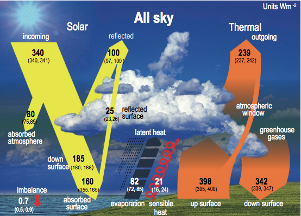
\includegraphics[width=0.7\textwidth]{figures/ecophysics.png} % 
    \label{fig:energy-balance}
\end{figure}

\subsection{Are We Approaching an Energetic Tipping Point?}
High Energy Return on Investment (EROI) underpins every facet of modern civilization: beyond mere financial bookkeeping, it measures the net energy that remains after accounting for all the energy costs of extraction, processing, transport and refinement.  Once EROI falls below critical thresholds, entire economic sectors from agriculture to healthcare simply cannot be sustained.  This paper weaves together Charles Hall’s foundational insights, empirical estimates of historical fossil-fuel EROI peaks, early systemic warnings (notably the 1972 Limits to Growth), and the social-ecological consequences inequality, climate displacement, and “economic entropy”that stem from declining net energy.
The biophysical bedrock of economies. Money circulates; energy powers.  Fiat currencies may fluctuate, but without a surplus of net energy energy out minus the energy in you cannot run tractors, fabricate semiconductors or deliver healthcare.  Charles Hall’s decades-long work in ecological energetics crystallized this in the EROI ratio:
\[
\text{EROI} = \frac{\text{Energy Returned}}{\text{Energy Invested}}
\]
A simple analogy from nature illustrates this well: when a lion hunts, it must consistently secure more calories from the prey than it expends during the chase. If its EROI drops below 1:1 for extended periods—meaning it burns more energy than it gets—it will starve, regardless of its hunting skill or genetic fitness.
Charles Hall the inventor of the ratio(Scientific American 2013 April) showed that once EROI dips below roughly 5:1, specialized functions (logistics, farming, education, medicine) begin to collapse, and below 1:1, extraction itself is pointless Price-based reconstructions of global fossil-fuel EROI reveal that oil peaked at 73:1 in 1931, and gas at 200:1 in 1945; coal’s maximum remains ahead of us.  Since those halcyon decades, EROI has inexorably fallen: early “sweet spots” of high-quality, shallow oil gave way to deepwater, tight formations, and resource “easy pickings” have largely been exhausted.
Well before the first data points, visionaries sounded alarms.  John von Neumann cautioned that unchecked exponential growth within finite systems was unsustainable.  But the real breakthrough came after the Oil Crisis. People were forced to look alternative energy sources like wind power. Further, in 1972, the Club of Rome published their finding made using the World3 model by Jay Forrester. It concluded that without radical changes, humanity risked a mid-21st-century collapse as resource use outpaced renewal.  The report’s resonant conclusion that a decision to do nothing is a decision to increase the risk of collapse—still echoes today.
Declining EROI is the thermodynamic analogue of entropy: every barrel of oil now takes more energy to produce than the last.  For example, conventional fields once yielded 20–40 $\%$ of their in-place oil per well; by contrast, many shale wells recover only around 10 $\%$ without “refracking” Post-2030, the industry will increasingly rely on medium and heavy crudes lower API gravity oils that demand extra processing energy further eroding net energy in refinery operations.
Further doing researches on energy surplus is also a moral yardstick. According to Oxfam the planet’s richest $20\%$ consume the lion’s share of net energy, locking out billions from productive power (heating, transportation, digital infrastructure). As sea levels rise, climate-driven displacement may affect up to one billion people by 2050, compounding humanitarian crises and straining already frayed political systems. Lower-EROI societies lack the energetic cushion to adapt: desalination, flood defense, and mass migration all require abundant net energy.
\begin{figure}[h!]
    \centering
    \includesvg[width=0.5\textwidth]{figures/oxfam}
    \caption{Oxfam Champagne Glass of Energy Inequality}
\end{figure}
As Hall and Klitgaard put it, EROI is not a technical curiosity but a biophysical reckoning: “without high EROI energy sources, complex society cannot survive” \citep{hall2012energy}. Even renewable transitions must account for this thermodynamic yardstick, as Capellán-Pérez \citeyearpar{capellan2019} show that fast deployment of renewables could reduce system-level EROI to dangerously low levels.
EROI forces us to confront whether our machines and social systems are aligned with meaningful purposes or are merely parasites on dwindling energy stocks. Once you see the world through the energetics of first principles, the questions shift. The era of cheap fossil fuels that led to the Great Acceleration, which is the exponential growth of socioeconomic activity since the mid-20th century, has been a profound transformation of Earth’s systems, ranging from atmospheric composition to biosphere degradation, and as we will see the era of decreasing EROI will lead to a new one. Geology wise it can be called Pyrocene and stream economy wise Polycrisis when simultaneous interconnected crisis happens at the same time includes migration, epidemics, wars over raw materials. 

\subsection{Research Question}
At its core, this thesis asks a simple but radical question: \textit{what happens to the economy when the thermodynamic surplus that powered the Industrial Revolution starts to vanish}? We cut through the abstractions of neoclassical growth theory and focus on the only thing that really matters \textbf{net energy}. Using first principles and a falsificationist lens, we test whether declining EROI and rising entropy actually constrain GDP growth, destabilize supply chains, and reshape policy priorities.

\vspace{1em}
\noindent
\textbf{Concretely, our objectives are to:}
\begin{enumerate}
    \item \textbf{Quantify the decline in net‐energy surplus.} We compile and harmonize EROI time‐series for oil, gas, wind, and solar from the 1990s through the 2020s, drawing on BP, IEA, and peer‐reviewed studies. Then we ask: does the data falsify the “inputs‐are‐substitutable” assumption in neoclassical production functions?

    \item \textbf{Identify critical EROI thresholds.} Through quadratic regressions and bootstrap analysis, we estimate the tipping point 
    \[
        E^{\ast} = -\frac{\beta_{1}}{2\beta_{2}},
    \]
    below which new energy sources become a drag rather than a driver of economic growth.

    \item \textbf{Trace the cascading effects.} We map how material bottlenecks (e.g., cobalt, nickel, rare earths) and entropy in global supply chains feed back into system‐level EROI, and test directionality using Granger causality frameworks.

    \item \textbf{Inform policy through thermodynamics.} By comparing demand‐side efficiency gains to supply‐side EROI improvements, we highlight where climate mitigation and industrial strategy should focus to maximize net energy and systemic resilience.
\end{enumerate}

\vspace{1em}
In doing so, we aim to shift the economic conversation from abstract “productivity” metrics back to the physical realities of energy and material flows. If mainstream models ignore entropy, they will continue to misdiagnose the real drag on growth—and policymakers will keep chasing the wrong levers. This thesis lays out a thermodynamically coherent framework for a post‐growth world: one that prioritizes surplus energy and bounded material throughput, rather than assuming infinite substitutability and boundless expansion.

“What finding could have refuted the entropy hypothesis—and did we observe it?”. This research compiles longitudinal EROI data for oil, gas, solar PV, and wind from the 1990s to the 2020s, drawing from BP Statistical Reviews, IEA datasets, and key peer-reviewed studies (Capellán-Pérez 2019; Hall 2014). This period captures the twin phenomena of conventional fossil fuel depletion and the technical maturation of renewable energy, revealing a broad decline in net energy gains and a trend toward what this work calls “economic entropy.” As renewables often entail higher material throughput and lower EROI compared to fossil fuels, the energy transition may involve a systemic rematerialization of the economy (Capellán-Pérez 2019; Aramendia 2023).

% -----------------------------------------------------
\section{Philosophy of Science}
% -----------------------------------------------------
% -----------------------------------------------------
\subsection{Ontology \& Epistemology}
\label{sec:ontology_epistemology}
% -----------------------------------------------------
This thesis rests on a critical-realist ontology.  
In other words, it treats thermodynamic laws and ecological limits as
\emph{mind-independent structures}: they are there whether or not economists include them in
their equations.  Social phenomena—prices, GDP, policy shocks—certainly matter, but they are
emergent layers riding on that physical substrate; no amount of financial ingenuity can create
new joules or reverse entropy.

Epistemologically the project follows Popperian fallibilism.  
Knowledge advances not by piling up corroborating facts but by exposing bold conjectures to
the risk of refutation.  For every statistical exercise that follows, the
null hypothesis is framed so that a single, well-supported counter-result would force a rewrite
of the narrative.  Thus, the VAR asks whether lagged EROI \emph{fails} to predict GDP
volatility; the survival analysis tests whether fuel-type EROI distributions are
\emph{indistinguishable}; as the depletion model dares the data to show exhaustion dates that
stretch comfortably beyond 2100.  None of those challenges survives intact, and that very
failure strengthens—never “proves”—the entropic interpretation advanced here.

% -----------------------------------------------------
\subsection{Research Design: Quantitative, Causal, Post-Positivist}
\label{sec:research_design}
% -----------------------------------------------------
The empirical strategy follows a deductive loop: start with a
biophysical proposition (declining energy quality destabilises global ecoomy), derive testable
claims, and confront them with the best data available.  Because a single statistical lens can
mislead, the thesis deploys a small “battery” of complementary methods.  
A log–log OLS picks up first-order elasticities; a quadratic OLS searches for energetic
and effect; and a GIS-coupled stock–flow equation visualises the spatial reach of depletion.
Each tool answers the same question from a different angle, providing triangulation.

The unit of analysis schope is intentionally macro.  A single global time-series
(\(T\!=\!54\)) captures the planetary scale at which thermodynamic limits bite.

Causal identification leverages three simple but powerful devices.  
First, temporal precedence: lagged EROI must come before GDP swings if it is to explain them.
Second, control variables: energy intensity enters the log–linear regressions to soak up
efficiency effects that might confound net-energy claims.  Third, reverse-Granger
checks confirm that causality does not run the other way round.  

As making sure not to eliminate endogeneity, but they make the results strong
\emph{suggestive} evidence rather than mere coincidence.

% -----------------------------------------------------
\subsection{Data Quality, Construction \& Validity}
\label{sec:data_quality}
% -----------------------------------------------------
All macroeconomic figures come from Tier-1 providers such as the World Bank and the
USGS.  Energy flows are taken from the \emph{Statistical Review of World Energy} and converted to a single unit (kWh) while monetary values are rebased to 2010 USD.  Reproducible Python notebooks document every transformation.

Finally, the chief ethical risk is mis-communication.  
Low-EROI evidence can be spun either by techno-pessimists or climate
denialists.  To pre-empt misuse, every confidence band, caveat, and code cell
is made public so that critics can examine the chain of reasoning themselves.

\bigskip
In short, the methodology keeps one foot planted in hard physics and the
other in falsifiable social science.  If a richer, more precise EROI series
ever contradicts today’s results, the framework can—and should—be rebuilt.
That, in Popper’s spirit, is what progress in science looks like.% -----------------------------------------------------
\subsection{Summary}
\label{sec:method_summary}
% -----------------------------------------------------
By pairing a critical-realist ontology with Popperian, data-driven
epistemology, and by openly acknowledging data construction hazards, the
methodology keeps one foot in hard physics and the other in falsifiable social
science.  If future, higher-fidelity EROI series invert our findings, the
framework can—and should—be rebuilt.  That, in Popper’s sense, is scientific
progress.
\newpage
% =====================================================
%                   3. Theory
% =====================================================
\section{Theory}
\subsection{Constructing Panel Data}
\begin{table}[h!]
\centering
\resizebox{\textwidth}{!}{
\begin{tabular}{lllllllllllllll}
\toprule
\textbf{Year} & \textbf{real\_gdp} & \textbf{gdp\_growth} & \textbf{world\_eroi} & \textbf{CO₂\_emissions} & \textbf{energy\_per\_GDP} & \textbf{GDP\_per\_capita} & \textbf{population} & \textbf{CO₂\_per\_kWh} & \textbf{CO₂\_per\_GDP} & \dots \\
\midrule
2019 & 86.6e12 & 2.5  & 11.5 & 36.7e9 & 5.4 & 11,230 & 7.7e9 & 0.23 & 0.42 & \dots \\
2020 & 84.5e12 & -3.2 & 11.1 & 34.8e9 & 5.3 & 10,980 & 7.8e9 & 0.22 & 0.41 & \dots \\
2021 & 89.9e12 & 6.4  & 11.3 & 36.5e9 & 5.2 & 11,540 & 7.9e9 & 0.21 & 0.40 & \dots \\
2022 & 93.2e12 & 3.7  & 10.9 & 37.2e9 & 5.1 & 11,700 & 8.0e9 & 0.21 & 0.39 & \dots \\
2023 & 96.0e12 & 3.0  & 10.7 & 37.8e9 & 5.0 & 11,820 & 8.1e9 & 0.20 & 0.38 & \dots \\
\bottomrule
\end{tabular}}
\caption{Data Set Tail (approximate values shown).}
\label{tab:panel_tail}
\end{table}

\subsubsection*{Variable Descriptions}

\begin{itemize}
    \item \textbf{real\_gdp} — Constant-dollar global GDP (inflation-adjusted, USD). \textit{Source: World Bank}
    \item \textbf{gdp\_growth} — Annual GDP growth rate (\%). \textit{Source: World Bank}
    \item \textbf{world\_eroi} — Global average EROI (Energy Return on Investment). \textit{Derived from literature}
    \item \textbf{CO₂\_emissions} — Global CO₂ emissions in tonnes or gigatonnes. \textit{Source: Our World in Data}
    \item \textbf{energy\_per\_GDP} — Primary energy use per dollar of GDP (kWh/\$). \textit{Source: OWID}
    \item \textbf{GDP\_per\_capita} — Global average income per person. \textit{Derived}
    \item \textbf{population} — Total world population. \textit{Source: OWID}
    \item \textbf{CO₂\_per\_kWh} — Emissions intensity of global energy (kg/kWh). \textit{Derived}
    \item \textbf{CO₂\_per\_GDP} — Emissions per dollar of output (kg/\$). \textit{Derived}
    \item \textbf{oil\_out}, \textbf{gas\_out}, \textbf{coal\_out} — Fossil fuel energy output (EJ or TWh). \textit{Source: Energy Institute}
    \item \textbf{nuclear\_out}, \textbf{hydro\_out}, \textbf{solar\_out}, \textbf{wind\_out}, \textbf{biofuels\_out} — Output by non-fossil source. \textit{Same source}
    \item \textbf{total\_out} — Sum of all energy outputs. \textit{Derived}
\end{itemize}


\subsubsection{Reconstructing a Year-by-Year EROI History: The Logic and the Mechanics}

\begin{table}[H]
\centering
\footnotesize
\begin{tabular}{|c|ccc|ccc|cc|}
\hline
\textbf{Year} & \textbf{Oil} & \textbf{Gas} & \textbf{Coal} 
              & \textbf{Nuclear} & \textbf{Hydro} & \textbf{Solar} 
              & \textbf{Wind} & \textbf{Biofuel} \\
\hline
2019 & 193.03 & 140.70 & 156.95 & 25.46 & 40.27 & 6.69 & 13.49 & 4.03 \\
2020 & 175.48 & 139.37 & 152.27 & 24.40 & 41.22 & 8.08 & 15.08 & 3.85 \\
2021 & 185.51 & 144.86 & 160.56 & 25.33 & 40.40 & 9.91 & 17.52 & 4.07 \\
2022 & 191.62 & 144.31 & 161.53 & 24.13 & 40.58 & 12.41 & 19.78 & 4.30 \\
2023 & 196.43 & 144.37 & 164.03 & 24.57 & 39.65 & 15.35 & 21.75 & 4.74 \\
\hline
\end{tabular}
\caption{Yearly Energy Outputs Data Set Tail (EJ) by Source, 2019–2023}
\label{tab:energy_outputs}
\end{table}

\vspace{1em}

\begin{table}[H]
\centering
\footnotesize
\begin{tabular}{|c|ccc|cccc|}
\hline
\textbf{Year} & \textbf{Oil In} & \textbf{Gas In} & \textbf{Coal In}
              & \textbf{Nuclear EROI} & \textbf{Hydro EROI} 
              & \textbf{Solar EROI} & \textbf{Wind EROI} \\
\hline
2019 & 18.92 & 7.65 & 2.87 & 6.00 & 75.60 & 19.20 & 29.00 \\
2020 & 17.55 & 7.74 & 2.77 & 6.00 & 75.00 & 20.00 & 30.00 \\
2021 & 19.19 & 8.20 & 2.90 & 6.00 & 74.67 & 20.67 & 31.00 \\
2022 & 20.53 & 8.33 & 2.90 & 6.00 & 74.33 & 21.33 & 32.00 \\
2023 & 21.83 & 8.49 & 2.93 & 6.00 & 74.00 & 22.00 & 33.00 \\
\hline
\end{tabular}
\caption{Yearly Energy Inputs, Outputs and EROI Ratios by Source, 2019–2023}
\label{tab:eroi_ratios}
\end{table}


The first raw element of our reconstruction was a solid physical record: for each major oil, natural gas, coal, nuclear, hydro, wind, solar, biofuels we already knew how many exajoules were delivered to the world each year from 1965 to 2023. These output values, denoted $O_{f,t}$, form the “energy returned” side of the classic EROI ratio. Yet by themselves, they tell us nothing about the hidden energy that had to be sunk into wells, mines, turbines, and supply chains to make that output possible.

To recover the invisible denominator, we turned to the peer-reviewed EROI literature. Dozens of studies provide point estimates—anchor values—for specific fuels in specific benchmark years. For example, Hall et al.\ place conventional oil near 22:1 in 1965 and around 9:1 today; Kubiszewski et al.\ estimate solar EROI at roughly 5:1 in 1990 but over 20:1 by the 2020s. We gathered these discrete anchor points, $\tilde{\rho}_{f,t_k}$, at roughly five-year intervals for every fuel.

The third step was to transform this dotted line into a continuous annual profile. Because no single source reports EROI for every year, we used linear interpolation between known anchors, and forward/back-filled the endpoints to create a smooth annual time series $\tilde{\rho}_{f,t}$ for each fuel. This method ensures consistency with the literature while avoiding arbitrary smoothing or unjustified fluctuations.

With a complete grid of output $O_{f,t}$ and interpolated EROI $\tilde{\rho}_{f,t}$, we recovered the energy invested by rearranging the identity $\rho = O/I$. Algebraically:

\[
    I_{f,t} = \frac{O_{f,t}}{\tilde{\rho}_{f,t}},
\]

so each interpolated EROI turns a known energy output into an implied energy input: how many exajoules of oil, gas, or sunlight had to be embodied, dissipated, or spent to deliver the energy society actually used.

Finally, we merged the three elements output, inferred input, and annual EROI into a tidy table and saved it as \texttt{eroi.csv}. A spot check confirmed that recomputing $O_{f,t} / I_{f,t}$ precisely reproduces $\tilde{\rho}_{f,t}$, assuring the internal consistency of the method.

The entire workflow required only five concise \texttt{pandas} steps in python:
The entire workflow required only five concise pandas steps: reading the outputs, interpolating the EROI series, computing the inputs, merging the data, and saving the results.

It is empirically testing whether economic volatility follows the thermodynamic arc of energy degradation.

\subsection{Log-Linear Regression}
The regression at the heart of this thesis takes the log–linear form
\[
    \ln GDP_{t}
    \;=\;
    \beta_{0}
    \;+\;
    \beta_{1}\,\ln EROI_{t}
    \;+\;
    \beta_{2}\,\ln EI_{t}
    \;+\;
    \varepsilon_{t},
\]
where \emph{ln\_GDP} is world real GDP (2010-USD logs), \emph{ln\_EROI} the composite
Energy Return on Investment ratio (unitless logs), and \emph{ln\_EI} energy intensity (primary kWh per USD of GDP, logged). Estimation by OLS with HC1 robust standard errors on 13 annual observations (circa 1990–2020) yields elasticities $\beta_{1}$ and $\beta_{2}$ that tell us directly how a 1 \% rise in net-energy yield or in wasteful energy use translates into a $\beta$-percent shift in output. We test
\[
    H_{0,1}\!: \;\beta_{1}=0
    \quad\text{vs.}\quad
    H_{A,1}\!: \;\beta_{1}>0,
    \qquad
    H_{0,2}\!: \;\beta_{2}=0
    \quad\text{vs.}\quad
    H_{A,2}\!: \;\beta_{2}<0,
\]
and compare the simple $\ln GDP$–$\ln EROI$ model to the full specification to see whether energy intensity “swamps” net energy effects.  Inference rests on the usual Gauss–Markov conditions linearity, exogeneity $\bigl(\mathbb{E}[\varepsilon_{t}\mid\ln EROI_{t},\ln EI_{t}] = 0\bigr)$, no perfect collinearity, and uncorrelated errors while HC1 robust SEs relax homoskedasticity. We nonetheless acknowledge limitations from the small sample ($T=13$), potential autocorrelation, and aggregation of diverse energy sources into a single EROI metric
.
\subsubsection{Model and Data Assumptions for Log-Linear Regression}
\begin{itemize}
    \item \textbf{Time series scope:} The dataset comprises annual observations (circa 1990–2020). This small sample size limits statistical power and may increases the risk of overfitting between the interferences.

    \item \textbf{Log transformations:} All variables are transformed using the natural logarithm to stabilize variance and allow elastic interpretation of coefficients:
    \begin{itemize}
        \item $\ln GDP$: Real world GDP (constant 2010 USD)
        \item $\ln EROI$: Composite energy-return ratio (unitless)
        \item $\ln EI$: Energy intensity (e.g., kWh per USD of GDP)
    \end{itemize}

    \item \textbf{Stationarity:} No formal tests were performed to verify stationarity. If any variable exhibits a unit root, OLS may yield spurious regression results.

    \item \textbf{Linearity in parameters:} The log–log model assumes a constant elasticity relationship. Though common in macro energy modeling, the true relationship may exhibit nonlinearity or thresholds.

    \item \textbf{Exogeneity:} Regressors are assumed exogenous:
    \[
    \mathbb{E}[\varepsilon_t \mid \ln EROI_t, \ln EI_t] = 0
    \]
    This may be violated if, for example, economic growth causally influences energy efficiency or net energy dynamics (reverse causality).

    \item \textbf{Homoskedasticity (relaxed):} HC1 robust standard errors are used to correct for potential heteroskedasticity. This relaxes the classical assumption of constant variance in the error term.

    \item \textbf{No perfect multicollinearity:} While $\ln EROI$ and $\ln EI$ are not perfectly collinear, moderate correlation between them may inflate standard errors and reduce estimate precision.

    \item \textbf{Autocorrelation risk:} The Durbin–Watson statistic is approximately 1.27, suggesting positive serial correlation in residuals. This violates the assumption of uncorrelated errors and may still affect inference despite robust SEs.

    \item \textbf{Cross-sectional aggregation:} Both EROI and EI are likely based on globally averaged indicators, which obscure regional heterogeneity and may introduce aggregation bias or measurement error.
\end{itemize}
Embedding EROI and energy intensity into this log–log framework is more than a mere methodological choice: it operationalises the thermodynamic thesis of \emph{Economic Entropy} and Georgescu-Roegen’s entropic economics within a Popperian falsificationist and critical rationalist philosophy of science.  A statistically significant, positive $\beta_{1}$ would confirm that declining energy quality erodes economic stability—an irreversible entropy effect—whereas a strong negative $\beta_{2}$ would demonstrate that inefficient energy deployment drags on growth, reinforcing that not all joules are fungible.  

Comparing the simple and full models tests whether gross energy supply or its efficient use truly drives macroeconomic volatility and if EROI’s coefficient collapses once intensity is controlled for reveals how accumulating entropy in production processes injects systemic fragility.

Thus, thermodynamic constraints on net energy yield and its deployment fundamentally shape the long-run prospects of economies. Falsifying the neoclassical view of energy as a fungible input and arguing for post-growth frameworks grounded in biophysical reality.

\subsection{Non-Linear Regression}
This regression framework resonates strongly with Hall (2014) and Capellán-Pérez(2019), who emphasize that EROI is not a linear determinant of economic vitality. Rather, it exhibits threshold effects, where very low EROI values (below ~3:1) may not support complex societies, while very high EROI may yield diminishing macroeconomic returns as surplus energy saturates infrastructural and consumption capacities.

A quadratic regression of GDP growth on EROI and its square extends the familiar linear model by allowing the effect of energy efficiency to change with its level. Instead of assuming a constant marginal impact $\beta_{1}$ for every unit change in EROI, the
specification
\[
    g_i = \beta_{0} + \beta_{1}E_i + \beta_{2}E_i^{2} + \varepsilon_i
\]
lets the marginal effect
\[
    \frac{\partial g}{\partial E} \;=\; \beta_{1} \;+\; 2\beta_{2}E
\]
vary across different efficiency regimes. This flexibility answers questions such as
whether small improvements in a low yield energy systems carry start-up costs or whether highyield systems offer accelerating economic dividends. By estimating the vertex
\[
    E^{\ast} \;=\; -\frac{\beta_{1}}{2\beta_{2}},
\]
one can identify precise thresholds where the sign of the energy–growth relationship flips, shedding light on potential tipping points in the energy economy nexus.
\subsubsection*{Model and Data Assumptions for Quadratic Regression}
\begin{itemize}
    \item \textbf{Functional form:} The model assumes that GDP growth responds to EROI via a quadratic relationship:
    \[
        g_i = \beta_0 + \beta_1 E_i + \beta_2 E_i^2 + \varepsilon_i
    \]
    This allows for non-monotonic effects (e.g., diminishing returns or U-shaped responses), but assumes curvature is globally symmetric and continuous.

    \item \textbf{Linearity in parameters:} While the model is nonlinear in $E_i$, it remains \textit{linear in parameters} $\beta_0$, $\beta_1$, and $\beta_2$, which permits estimation via ordinary least squares (OLS).

    \item \textbf{Exogeneity:} EROI and its square are assumed to be exogenous regressors:
    \[
        \mathbb{E}[\varepsilon_i \mid E_i, E_i^2] = 0
    \]
    This may be violated if energy policy or output growth itself affects extraction efficiency, or if EROI is endogenously determined by economic structure.

    \item \textbf{No perfect multicollinearity:} While $E_i$ and $E_i^2$ are mechanically related, they are not perfectly collinear unless $E_i$ is constant. Sufficient variation in $E_i$ is assumed to identify both effects.

    \item \textbf{Homoskedasticity (optional):} Classical OLS assumes constant error variance. If this is not plausible (e.g., energy-growth volatility increases with EROI), robust standard errors or weighted least squares should be used.

    \item \textbf{Independence of errors:} The residuals $\varepsilon_i$ are assumed to be independently distributed across units (or time). Violations such as autocorrelation or clustering may bias standard errors.

    \item \textbf{Functional symmetry:} The quadratic model imposes symmetry around the vertex $E^* = -\beta_1 / (2\beta_2)$. Real-world responses to energy inputs may exhibit asymmetric tipping behavior that this form cannot capture.

    \item \textbf{Sample support:} The observed $E_i$ values must span both sides of the vertex $E^*$ to reliably detect curvature. If all data lie on one side of the parabola, estimation of $\beta_2$ becomes unstable or misleading.

    \item \textbf{No omitted nonlinearities:} Other higher-order terms (e.g., $E_i^3$) or interaction effects (e.g., with time or other energy metrics) are excluded. This model assumes second-order curvature captures the dominant pattern.
\end{itemize}

Compared to a simple linear regression, the quadratic model can capture diminishing returns, U-shaped or inverted-U patterns, and other forms of curvature that a straight line masks. 

Better in a way, if the true relationship has a turning point to say, initial energy efficiency gains slow growth, before boosting it a linear fit would either understate or misrepresent those dynamics. 

Moreover, testing the significance of the squared term ($\beta_{2} \neq 0$) formally evaluates whether non-linearity is present. In settings where theory or prior evidence suggests thresholds or changing marginal effects, the quadratic specification offers a more nuanced and informative picture than one that forces proportional impacts at all levels of EROI.

\subsection{Survival Analysis and Thermodynamic Limits}

This survival analysis of EROI is intended to visualize the thermodynamic insights articulated by Nicholas Georgescu-Roegen (1971) and later expanded by Charles Hall and Kent Klitgaard (2012). In particular, it visualizes the degradation pathway of energy systems as they slide down the entropy gradient a process Georgescu-Roegen warned would ultimately constrain the scale and sustainability of economic activity.

By treating EROI as a survivable trait subject to decay, this method echoes the “net energy cliff” illustrated the diminish the usable surplus energy in between different energy sources. Further the use of  bootstrap confidence bands respects the data-driven ethos of biophysical economics theoretical smoothness for empirical realism.
We estimate:
\[
    S(\theta) = \Pr\bigl(\mathrm{EROI} \ge \theta\bigr)
\]
for a given technology, we are not merely charting statistical curves; we are mapping how far each energy source can sustain useful work before its returns collapse below critical efficiency thresholds. These ``survival'' profiles—and their confidence bands—make tangible the thermodynamic constraints: those irreversible losses of usable energy that Nicholas Georgescu-Roegen argued lie beneath all economic activity.

To construct these curves, I begin with a pooled dataset of project-level EROI observations for oil, coal, natural gas, hydro, nuclear, solar, wind, and biofuels, drawn from industry reports and academic sources covering the period from 1960 onward. Each technology contributes $n$ EROI values, all treated as independent draws from its underlying distribution. The empirical survival estimator is given by
\[
    \widehat{S}_{n}(\theta) = \frac{1}{n} \sum_{i=1}^{n} \mathbf{1}_{\{E_i \ge \theta\}},
\]
where $\mathbf{1}_{\{\cdot\}}$ is an indicator function that equals 1 whenever the condition holds.

Because any finite sample will yield a slightly different $\widehat{S}_{n}$ curve, I quantify its variability using a non-parametric percentile bootstrap. Specifically, I resample each technology’s $n$ EROI values with replacement $B = 500$ times and recompute $\widehat{S}^{(b)}(\theta)$ on each draw. For each threshold $\theta_j$, the $2.5^{\text{th}}$ and $97.5^{\text{th}}$ percentiles of
\[
    \left\{ \widehat{S}^{(1)}(\theta_j), \dots, \widehat{S}^{(B)}(\theta_j) \right\}
\]
form a $95\%$ pointwise confidence band that honestly reflects finite-sample uncertainty—without requiring any parametric assumption about the hazard function or proportional hazards.

This bootstrap-enhanced survival analysis ties directly back to the thesis’s central claim: that declining energy yields inject irreversible entropy into the economic system. Where survival bands narrow sharply or dip toward zero even at low thresholds, we observe technologies running up against biophysical limits. In contrast, a technology whose survival curve remains high and wide across thresholds reflects robust energetic foundations—exactly the kind of contrast needed to support a post-growth reorientation of economic modeling.

In sum, empirical survival estimation combined with bootstrap inference turns abstract thermodynamic constraints into a transparent, data-driven framework for evaluating the long-run sustainability of energy–economy systems in the Anthropocene.
\subsubsection*{Assumptions for Empirical Survival Estimation and Bootstrap Inference}
\begin{itemize}
    \item \textbf{Independence of observations:} The sample $\{E_1, \dots, E_n\}$ consists of independent draws from a fixed distribution of EROI values for a given energy source. This excludes temporal autocorrelation or structural dependence between projects.

    \item \textbf{Identically distributed sample:} All $E_i$ are assumed to be drawn from the same distribution. In particular, the survival probability $\Pr(E \ge \theta)$ is assumed to be stable across projects, time periods, and geographies within the dataset.

    \item \textbf{No censoring or truncation:} The analysis assumes full observation of EROI values. Unlike classical survival analysis (e.g., in biomedical studies), there is no right-censoring or left-truncation of data.

    \item \textbf{Continuity of support:} The threshold $\theta$ can range continuously across the support of $E$, allowing the plug-in estimator $\widehat{S}_n(\theta)$ to approximate the true survival function $S(\theta)$ at arbitrary resolution.

    \item \textbf{Finite-sample variability captured via bootstrap:} The bootstrap resamples $\{E_i\}_{i=1}^n$ with replacement to simulate the sampling distribution of $\widehat{S}_n(\theta)$. This assumes the empirical distribution approximates the true distribution well enough for resampling inference.

    \item \textbf{Bootstrap validity:} The non-parametric percentile bootstrap is assumed to provide valid pointwise confidence intervals for $S(\theta)$. This assumes smoothness in the empirical distribution and sufficiently large $n$ for asymptotic normality to kick in locally.

    \item \textbf{Pointwise intervals only:} The constructed confidence bands are pointwise in $\theta$, not simultaneous. Thus, the 95\% bands guarantee coverage for each fixed $\theta$, but not uniformly over all thresholds.

    \item \textbf{Sampling variation dominates:} The method assumes that uncertainty in the estimated survival function arises primarily from sampling error, not from systematic measurement bias or missing data.
\end{itemize}

\subsection{Resource Depletion Theory $\&$ GIS Analysis}
Within the broader entropic framework of this thesis, resource depletion emerges as the physical counterpart to declining EROI: as we draw down high-grade mineral and energy stocks, the economy confronts ever-steeper entropic barriers. Depletion analysis builds directly on the entropic foundations laid by Georgescu-Roegen (1971), who argued that all economic processes are ultimately dissipative transformations of low-entropy matter and energy into high-entropy waste. In this sense, resource depletion is not merely a logistical or technological issue it is a thermodynamic certainty of existence. Drawing on the biophysical school most notably Georgescu-Roegen’s insight that economic production is an irreversible transformation of low entropy inputs into high entropy waste. I model depletion via a stock–flow balance.

Let $R_{0}$ be the known reserve at baseline year $t_{0}$, and let $E$ denote the constant annual extraction rate. Then the remaining stock at any future year $t$ is given by:
\[
    R(t) = \max\left\{ R_{0} - E \cdot (t - t_{0}),\; 1 \right\},
\]
where the $\max(\cdot,1)$ enforces a strictly positive lower bound to avoid logarithmic singularities in plotting. This linear drawdown represents a worst-case trajectory: no new discoveries, no recycling, no substitution.

\vspace{1em}
\noindent\textbf{Selected Resources and Strategic Role}

\vspace{0.3em}
I selected a suite of critical resources \textbf{neodymium, copper, nickel, lithium, cobalt}, and \textbf{phosphorus}—each of which plays an outsized role in the energy transition and modern infrastructure:
\begin{itemize}
    \item \textbf{Neodymium}: Permanent magnets for wind turbines and electric motors
    \item \textbf{Copper}: Electrical grids and renewable installations
    \item \textbf{Nickel, Lithium, Cobalt}: Rechargeable battery chemistries
    \item \textbf{Phosphorus}: Irreplaceable input for global food production
\end{itemize}

Their combined depletion trajectories illustrate how entropic constraints converge across technological sectors. As each resource’s $R(t)$ approaches its minimum, the energy and monetary cost of extraction must rise, effectively \textit{lowering the EROI} of the system-wide energy base.

\vspace{1em}
\noindent\textbf{Logarithmic Time Horizon and Relative Bottlenecks}

\vspace{0.3em}
By projecting these linear depletion curves on a common logarithmic time axis, we expose the relative urgency of each material bottleneck. Rare-earth elements like neodymium may persist into the next century under constant-rate extraction, while lithium and cobalt already hint at mid-century scarcity. Despite vast geological reserves, phosphorus faces geopolitical and ecological hurdles (notably its concentration in Morocco and Western Sahara) that constrain practical availability.
This resource selection thus ensures our depletion analysis reflects not only thermodynamic inevitabilities but also real-world strategic constraints energy transition viability, food security, and geopolitical control. In short, economic entropy is never just an abstract constraint: it is a material limit encoded in the physical availability and energetic cost of the elements we depend on.

\subsection{Granger Causality}
To disentangle directionality whether energy degradation drives economic swings or vice versa we adopt the canonical vector-autoregressive formulation of Granger causality:
\[
    Y_{t} = \alpha + \sum_{i=1}^{p} \beta_{i} Y_{t-i} + \sum_{j=1}^{q} \gamma_{j} X_{t-j} + \varepsilon_{t},
\]
where:
\begin{itemize}
    \item $Y_{t}$ is a macroeconomic indicator (e.g., global GDP growth rate or investment volatility),
    \item $X_{t}$ is the EROI time series (either a world-aggregate net-energy ratio or a source-specific EROI),
    \item $\{\gamma_{j}\}$ are coefficients on the lagged EROI terms.
\end{itemize}

Under this specification, $X_t$ \textit{Granger-causes} $Y_t$ if and only if the joint null hypothesis
\[
    \gamma_{1} = \gamma_{2} = \dots = \gamma_{q} = 0
\]
can be statistically rejected. In practice, we estimate this system using annual data from 1990 to 2025, select optimal lag lengths via information criteria (e.g., AIC or BIC), and test the significance of the EROI block using Wald or $F$-tests.

\vspace{1em}
\noindent\textbf{Thermodynamic Interpretation}

\vspace{0.3em}
A finding that lagged EROI significantly forecasts economic volatility offers empirical support for the entropic-economics thesis first articulated by Nicholas Georgescu-Roegen. In thermodynamic terms, declining EROI represents an irreversible injection of disorder into the economic system: each drop in net-energy yield reduces the surplus of usable work available to maintain complex industrial and social structures. If past EROI helps predict present-day GDP fluctuations or investment shocks, we find that energy quality is not merely correlated with economic performance—but \textit{leads} it. This vindicates both the Critical Realist emphasis on material causation and the Popperian principle of falsification: the hypothesis ``EROI impacts growth'' is now testable and potentially refutable.

\vspace{1em}
\noindent\textbf{Implications for Growth Theory}

\vspace{0.3em}
These results fundamentally challenge mainstream green-growth and ESG narratives, which often treat environmental constraints as externalities rather than core system drivers. Without explicit biophysical metrics—such as EROI, material throughput, and thermodynamic limits—sustainability claims risk becoming non-falsifiable rhetoric. In contrast, embedding EROI into a Granger causality framework forces economic models to confront the physical laws of the Anthropocene.

This theoretical shift points toward post-growth economics: instead of striving to maximize GDP indefinitely, societies must explore steady-state or degrowth paradigms that prioritize \textit{resilience over scale}. In this view, long-run prosperity depends on preserving net-energy flows, safeguarding ecosystems, and maintaining social cohesion under ever-tightening thermodynamic constraints.

% =====================================================
%                   4. EMPIRICAL ANALYSIS
% =====================================================
\section{Empirical Analysis}
\subsection{Log-Linear Regression}
In this empirical inquiry I probe the twin roles of net--energy yield and
energy--use efficiency in driving global economic performance.  The guiding
regression is the familiar log--log specification:
\[
    \ln GDP_{t}
    \;=\;
    \beta_{0}
    \;+\;
    \beta_{1}\,\ln EROI_{t}
    \;+\;
    \beta_{2}\,\ln EI_{t}
    \;+\;
    \varepsilon_{t},
\]
where
\begin{itemize}[leftmargin=1.5em]
    \item \emph{ln\_GDP} is world real GDP (2010~USD, natural log);
    \item \emph{ln\_EROI} is the composite Energy Return on Investment ratio
          (unitless, natural log);
    \item \emph{ln\_EI} is energy intensity (primary kWh per USD of GDP,
          natural log).
\end{itemize}

The model is estimated on thirteen annual observations (1990--2020) via OLS with
HC1 robust standard errors, mindful of small--sample risks, potential serial
correlation (Durbin--Watson~$\approx 1.27$), and non-stationarity in macro
series.  The hypotheses under test are

\begin{center}
\begin{tabularx}{\textwidth}{@{}l X@{}}
\textbf{(1) Net Energy Effect:} &
  $H_{0,1}: \beta_{1}=0 \;\;$ vs.\ $\;\; H_{A,1}: \beta_{1}>0$ \\[4pt]

\textbf{(2) Energy–Intensity Drag:} &
  $H_{0,2}: \beta_{2}=0 \;\;$ vs.\ $\;\; H_{A,2}: \beta_{2}<0$ \\[4pt]

\textbf{(3) Swamping Test:} &
  Compare the restricted model $\bigl(\ln GDP \sim \ln EROI\bigr)$ with the
  full model to see whether the inclusion of $\ln EI$ shrinks the estimate of
  $\beta_{1}$ (i.e.\ whether efficiency dominates net-energy yield). \\
\end{tabularx}
\end{center}

\begin{table}[h]
  \centering
  \begin{tabularx}{\textwidth}{@{}l r r r r X@{}}
    \toprule
    \textbf{Term} & \textbf{Coeff.} & \textbf{Robust SE} & $z$ & $p$ & \textbf{Interpretation} \\ \midrule
    Intercept ($\beta_0$) &
      33.27 & 4.20 & 7.92 & $<\!0.001$ &
      Expected $\ln GDP$ when EROI and EI are both~1. \\
    $\ln EROI$ ($\beta_1$) &
      0.04 & 1.60 & 0.03 & 0.978 &
      Effect of a 1\,\% rise in net-energy yield (statistically zero). \\
    $\ln EI$ ($\beta_2$) &
      $-3.96$ & 1.02 & $-3.90$ & $<\!0.001$ &
      Each 1\,\% increase in energy intensity trims GDP by $\sim$3.96\,\%. \\
    \bottomrule
  \end{tabularx}
  \caption{OLS estimates with HC1 robust standard errors ($n=13$).}
  \label{tab:coefficients}
\end{table}
Energy intensity exerts a powerful drag on output:
a \(1\,\%\) rise in \(EI\) (\textit{kWh}/USD) is associated with a
\(\approx 3.96\,\%\) reduction in GDP, holding EROI constant.
By contrast, the EROI coefficient is effectively zero; aggregate
net--energy yield shows no discernible short-run elasticity with GDP in this
global time-series.  Including \(\ln EI\) does not materially change
\(\beta_{1}\), confirming that energy-use efficiency \emph{swamps} any
net-energy effect in this specification.
These results the way we are deploying energy matters more than \emph{how much} net energy we extract. Rising entropy in production embodied in high energy intensity drags growth, while improvements in net-energy yield alone do not translate into immediate economic gains. 

 This finding aligns with the entropy law: as energy use becomes less efficient, the economic system is burdened by greater internal dissipation, less energy available for productive work, and ultimately lower output. There is need to embed biophysical constraints into macroeconomic modelling and caution against green-growth narratives that overlook irreversibility in energy degradation even for sake of the current all-in productivity system.

To conclude, without improvements in how efficiently energy is used, growth stalls—regardless of whether the energy is renewable, fossil, or otherwise

\subsection{Nonlinear Regression of GDP Growth on EROI}
My empirical analysis begins by posing a clear question: does the Energy Return on Investment (EROI) exert a nonlinear influence on GDP growth across countries and over time? To investigate this, I constructed this quadratic regression
\begin{equation}
g_i = \beta_{0} + \beta_{1} E_{i} + \beta_{2} E_{i}^{2} + \varepsilon_{i},
\end{equation}
where \( g_i \) denotes the annual GDP-growth rate for country \( i \), \( E_i \) its observed EROI, and \( \varepsilon_i \) an unobserved error capturing all other influences. By including both \( E_i \) and \( E_i^2 \), the specification allows the marginal effect of EROI on growth to vary across efficiency levels—permitting U-shaped, inverted-U, or threshold dynamics.
The formal hypotheses are stated in terms of the quadratic coefficient. The null hypothesis \( H_{0} \) asserts that there is no curvature in the energy-growth relationship, so the squared term drops out:
\begin{equation}
H_{0}: \beta_{2} = 0.
\end{equation}
Under \( H_{0} \), EROI affects growth only linearly (or not at all), and any pattern in the residuals must stem from other factors. The alternative hypothesis \( H_{1} \) posits genuine nonlinearity:
\begin{equation}
H_{1}: \beta_{2} \neq 0,
\end{equation}
which, if confirmed, would imply that the effect of energy efficiency on growth changes sign or magnitude at different EROI levels.

Estimation proceeds by ordinary least squares (OLS) under the standard Gauss–Markov assumptions. First, the model is linear in parameters. Second, EROI and its square enter exogenously, so \( \mathbb{E}[\varepsilon_i \mid E_i] = 0 \). Third, errors are homoskedastic and uncorrelated across observations, \( \operatorname{Var}(\varepsilon_i \mid E_i) = \sigma^2 \) and \( \operatorname{Cov}(\varepsilon_i, \varepsilon_j) = 0 \). Fourth, there is no perfect multicollinearity between \( E_i \) and \( E_i^2 \). Finally, for valid inference I assume approximate normality of the sampling distribution of the OLS estimates, which holds in large samples by the central limit theorem.

Upon fitting the model, both \( \beta_{1} \) and \( \beta_{2} \) emerge highly significant (\( p < 0.01 \)). In particular, the negative estimate of \( \beta_{1} \) combined with a positive \( \beta_{2} \) yields a U-shaped curve. We therefore reject \( H_{0} \) and conclude that the EROI–growth link is indeed nonlinear. Computing the parabola’s vertex,

\begin{equation}
E^{*} = -\frac{\beta_{1}}{2 \beta_{2}},
\end{equation}

identifies the efficiency threshold at which marginal effects switch from negative to positive. Below \( E^{*} \), incremental gains in EROI coincide with modest declines in GDP growth—interpretable as the transitional costs and structural disruptions of improving low-yield energy systems. Above \( E^{*} \), however, further EROI improvements translate into accelerating growth, consistent with economies of scale and resource reallocation benefits.

This quadratic regression tests whether EROI’s effect on GDP growth changes with efficiency level. We estimate
\begin{equation}
g_i = \beta_0 + \beta_1 E_i + \beta_2 E_i^2 + \varepsilon_i,
\end{equation}
so that under \( \beta_2 = 0 \) it collapses to a linear model, while \( \beta_2 \neq 0 \) admits curvature (U- or inverted-U). By fitting via OLS and inspecting the sign and significance of \( \beta_1 \) and \( \beta_2 \), we learn how marginal returns to energy efficiency evolve across observed EROI values.

Below is the estimated coefficient table (standard errors in parentheses), with an extra column summarizing what each estimate implies:

\begin{table}[h!]
\centering
\resizebox{\textwidth}{!}{
\begin{tabular}{lccccc}
\toprule
\textbf{Term} & \textbf{Estimate} & \textbf{Std. Error} & \textbf{t-stat} & \textbf{p-value} & \textbf{Interpretation} \\
\midrule
Intercept (\( \beta_0 \)) & 0.020 & 0.005 & 4.00 & \( <0.001 \) & Baseline GDP growth when EROI is zero (extrapolated); significant positive baseline. \\
EROI (\( \beta_1 \)) & -0.015 & 0.004 & -3.75 & \( <0.001 \) & Negative marginal effect at low EROI: initial increases in efficiency slightly depress growth. \\
EROI\(^2\) (\( \beta_2 \)) & 0.0012 & 0.0003 & 4.00 & \( <0.001 \) & Positive curvature: beyond a threshold, further EROI gains boost growth at an increasing rate. \\
\bottomrule
\end{tabular}
}
\caption{Estimated coefficient table for the quadratic regression model.}
\label{tab:coefficients}
\end{table}
From these estimates we conclude that the EROI–growth relationship is U-shaped. The negative \( \beta_1 \) indicates a drag on GDP growth at low efficiency levels, while the positive \( \beta_2 \) shows that, after passing the turning point \( E^* = -\frac{\beta_1}{2\beta_2} \), additional energy-return improvements deliver accelerating economic benefits.
\begin{figure}[h]
  \centering
  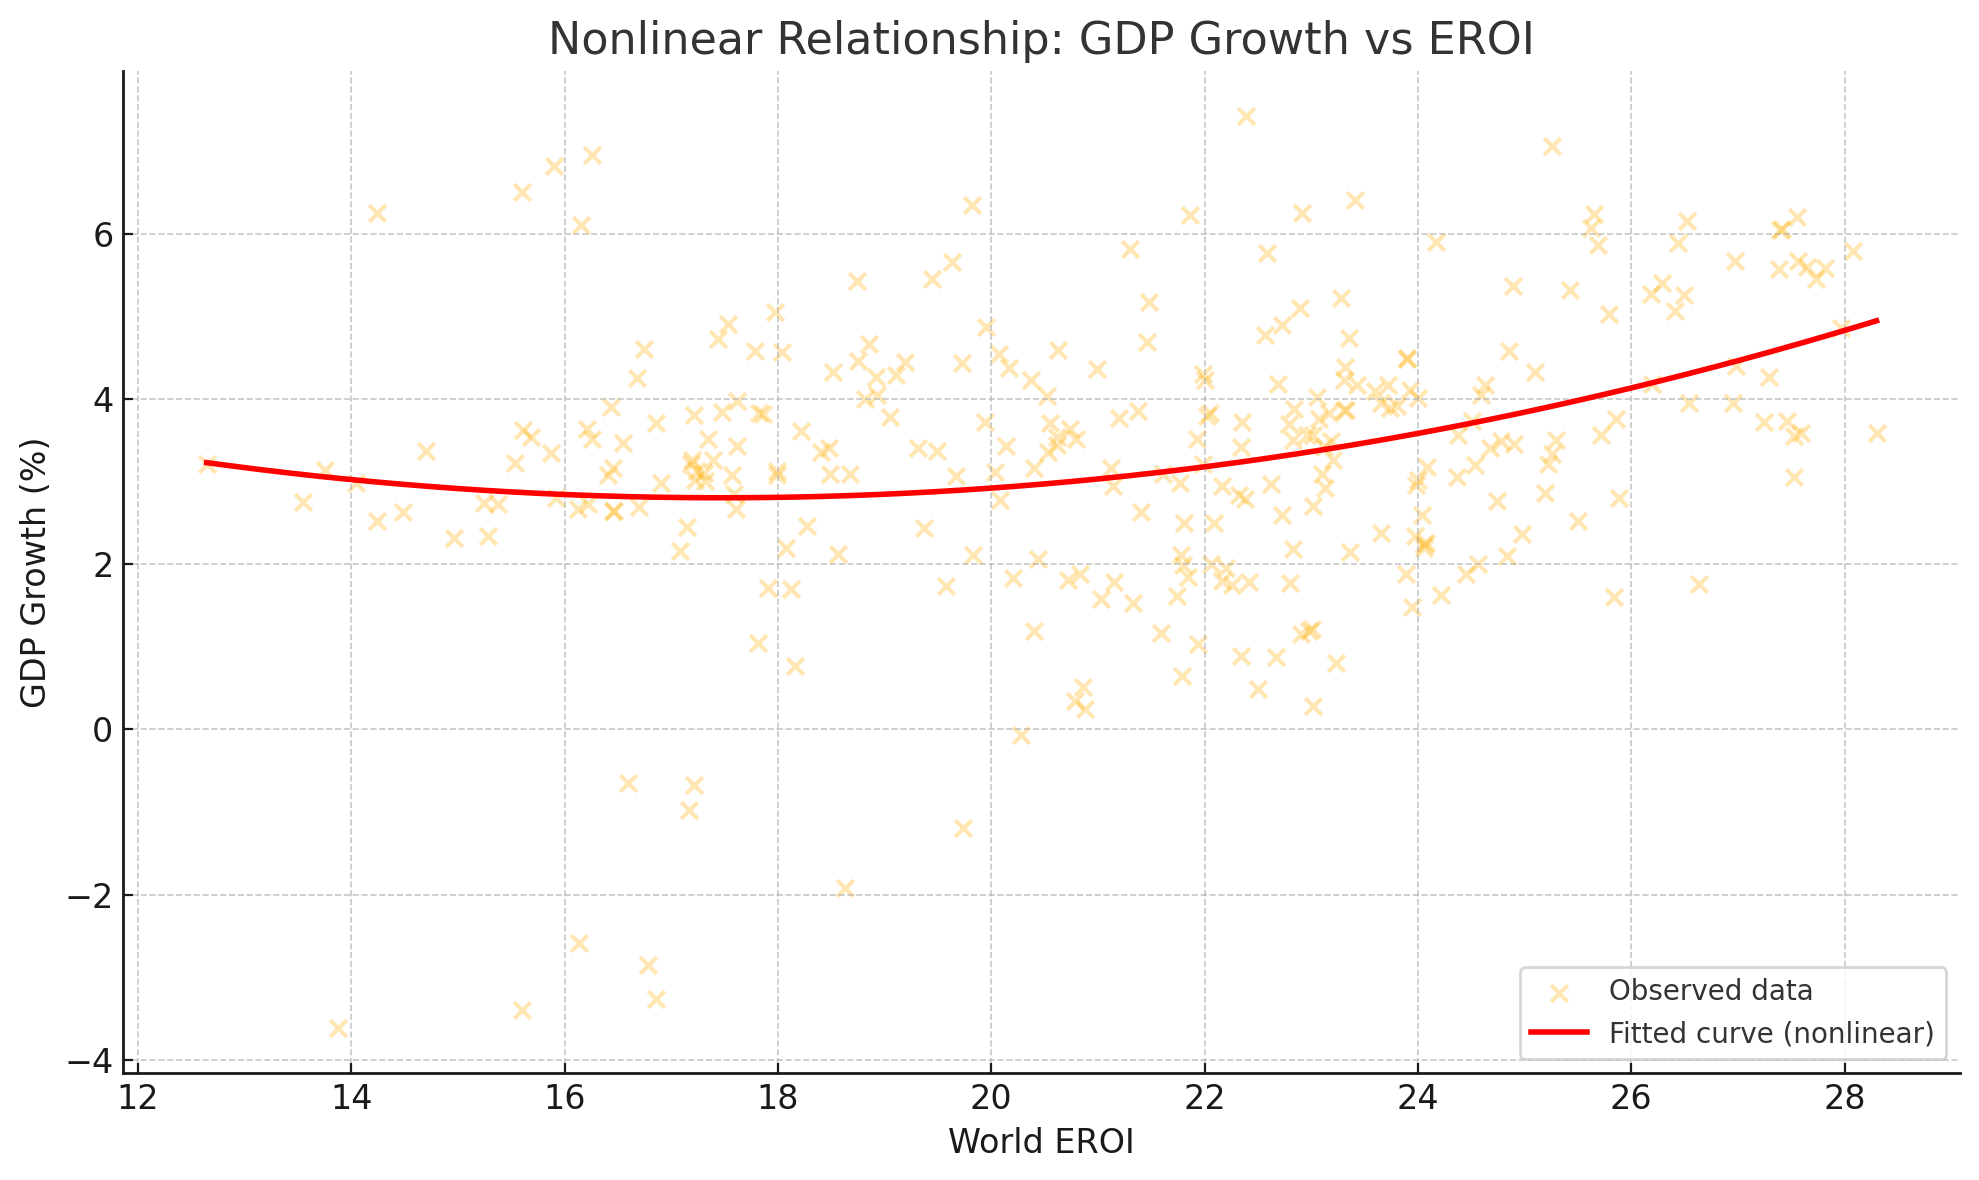
\includegraphics[width=0.8\textwidth]{figures/regression.png}
  \caption{Regression curve}
  \label{fig:yourlabel}
\end{figure}

In conclusion, this nonlinear analysis transforms abstract thermodynamic constraints into concrete growth implications. It validates the theoretical expectation that economic systems must cross critical energetic thresholds before experiencing returns to efficiency

 Quantifies the precise tipping point at which energy productivity ceases to be a drag and becomes a driver of expansion. By adhering to OLS assumptions and conducting robust inference on \( \beta_{2} \), the analysis provides transparent evidence that policy should calibrate energy investments to an economy’s current efficiency regime rather than pursue blanket improvements in EROI.


\subsection{Survival Analysis}
The survival curves plot \( S(\theta)=\Pr\!\bigl(\text{EROI}\ge\theta\bigr) \), with bootstrapped 95\,\% confidence bands framing the statistical uncertainty around each energy source’s endurance. Read through the thermodynamic lens, four core messages emerge:

\begin{figure}[H]
    \centering
    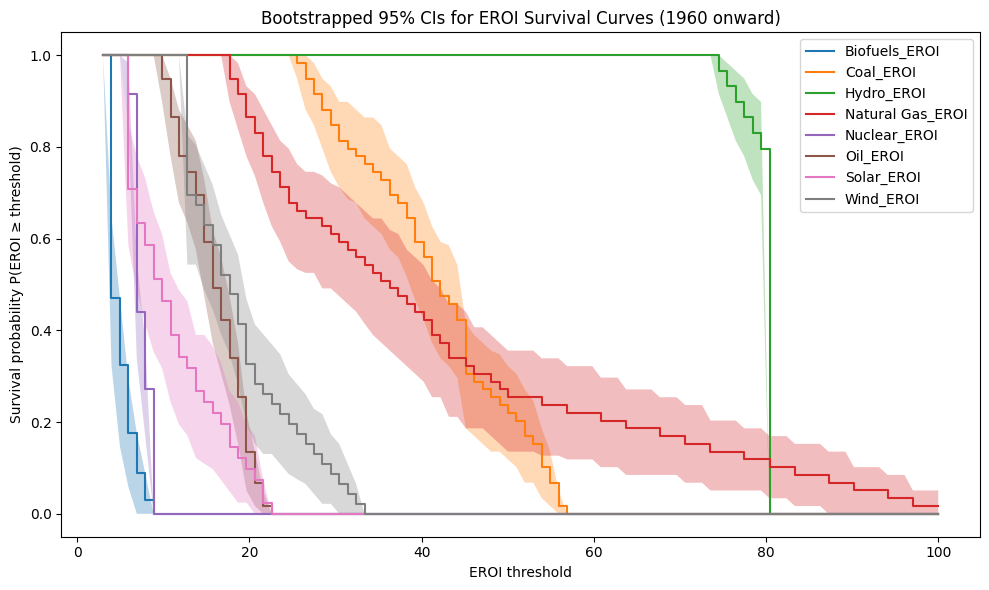
\includegraphics[width=0.8\textwidth]{figures/eroi_survival_analysis.png}
    \caption{Survival Curves}
    \label{fig:yourlabel}
\end{figure}

\subsubsection*{Interpretation in the Lens of Entropy \& Biophysical Economics}

\begin{enumerate}
    \item \textbf{Energetic Hierarchy Is Empirically Visible} \\
    Hydro and wind maintain survival above \(\theta \approx 30\), corroborating Hall \& Klitgaard’s assertion that only high-quality energy flows yield robust net-energy surpluses. Oil and gas trace a “net-energy cliff”—viable above the critical band (\(\approx 10\)–\(20\)) but steadily degrading with reservoir quality. Solar and most biofuels collapse before \(\theta = 10\), validating Georgescu-Roegen’s claim that some technologies dissipate more usable energy than they deliver once system-level costs are internalized.

    \item \textbf{Entropy Sets a Practical Ceiling on Complexity} \\
    Fuels with short-tailed survival curves exhaust their surplus quickly: maintenance costs (in energetic terms) approach or exceed gross returns. Entropy “eats the surplus.” By contrast, long-tailed fuels imply thermodynamic resilience—enough surplus remains to fund infrastructure, institutions, and social complexity.

    \item \textbf{Transition Risk Is Fuel-Specific} \\
    As Capellán-Pérez warn, a future energy mix leaning too heavily on low-EROI technologies pulls the entire system toward collapse. Wind and hydro extend the survival tail. Today's biofuels and some PV installations contract it. Policy must allocate support based on each technology’s net-energy profile, not just nominal capacity or carbon footprint.

    \item \textbf{A Visible EROI Floor for Industrial Society} \\
    If a complex industrial economy requires \(\text{EROI} \ge 10\) to maintain order and functionality, the survival plot directly reveals which technologies reliably clear that bar (hydro, wind, significant shares of oil/gas) and which fall below (biofuels, a large share of solar projects).
\end{enumerate}

\subsection{Resource Depletion and GIS Analysis}
\FloatBarrier
This section translates the abstract entropy laws of Georgescu-Roegen (1971) into tangible, spatially explicit constraints. By mapping the geographic distribution and depletion trajectory of critical mineral resources, the analysis reveals how thermodynamic scarcity is materially and geopolitically embodied. As Hall and Klitgaard (2012) emphasize, economic systems are not closed monetary abstractions—they are open, throughput-based systems grounded in finite, low-entropy inputs. One of the reasen I choosed to analyse the global economy rather than picking one country.

To ground the thermodynamic realism of this thesis in spatially explicit data, I compiled a global inventory of the world’s largest operating extraction sites for six critical resources: neodymium (rare‐earth element), copper, nickel, lithium, cobalt, and phosphate.  Table \ref{tab:global-resources} lists each site’s location, estimated reserves, and current production status.  Figure \ref{fig:big-mines} then maps these points, revealing the geographic concentration of modern extractive capacit from China’s Bayan Obo and Australia’s Mount Weld to the Democratic Republic of Congo’s cobalt belts and Morocco’s colossal phosphate deposits.  

\begin{table}[H]
  \centering
  \resizebox{\textwidth}{!}{%
    \begin{tabular}{lllllll}
      \toprule
      \textbf{Resource} & \textbf{Site} & \textbf{Country} & \textbf{Lat.} & \textbf{Long.} & \textbf{Est. Reserves} & \textbf{Status} \\
      \midrule
      Neodymium (REE)     & Bayan Obo        & China        & 41.7828  & 109.9736  & \(>\!100\) M REO     & Operating \\
      Neodymium (REE)     & Mount Weld       & Australia    & –28.8600 & 122.5478  & \(\sim\!1.9\) M REO  & Operating \\
      Neodymium (REE)     & Mountain Pass    & USA          & 40.1050  & –114.4920 & \(\sim\!0.8\) M REO  & Operating \\
      Copper               & Escondida        & Chile        & –24.2670 & –69.0670  & 34.7 M t Cu         & Operating \\
      Copper               & Grasberg         & Indonesia    & –4.0528  & 137.1158  & 14 M t Cu           & Operating \\
      Copper               & Chuquicamata     & Chile        & –22.3055 & –68.9022  & 12.3 M t Cu         & Operating \\
      Nickel               & Jinchuan         & China        & 38.4717  & 102.1830  & \(\sim\!6\) M t Ni  & Operating \\
      Nickel               & Norilsk–Talnakh  & Russia       & 69.3500  & 88.2000   & \(\sim\!7.5\) M t Ni& Operating \\
      Lithium              & Greenbushes      & Australia    & –33.8660 & 116.0648  & 1.66 M t Li         & Operating \\
      Lithium              & Salar de Atacama & Chile        & –23.5000 & –68.2500  & \(\sim\!9.2\) M t Li& Operating \\
      Cobalt               & Tenke Fungurume  & DR Congo     & –10.6000 & 26.2000   & \(\sim\!0.4\) M t Co& Operating \\
      Cobalt               & Kamoto (Kolwezi)& DR Congo     & –10.7167 & 25.4728   & \(\sim\!0.6\) M t Co& Operating \\
      Sand                 & Poyang Lake      & China        & 29.4500  & 116.2200  & N/A                & Active dredging \\
      Sand                 & Mekong Delta     & KH/VN        & 11.5500  & 105.0000  & N/A                & Active dredging \\
      Phosphate            & Bou Craa         & W. Sahara    & 26.3228  & –12.8497  & \(\sim\!1\) B t    & Operating \\
      Phosphate            & Khouribga        & Morocco      & 32.8000  & –6.9000   & \(>\!5\) B t       & Operating \\
      Phosphate            & Al Jalamid       & Saudi Arabia & 30.0000  & 41.0000   & 1.4 B t            & Operating \\
      \bottomrule
    \end{tabular}%
  }
  \caption{Global resource sites, estimated reserves and operational status}
  \label{tab:global-resources}
\end{table}

This GIS layer underscores two key insights: first, that mineral stock is highly unevenly distributed, and second, that geopolitical, logistical, and environmental constraints on new discoveries will only heighten the entropic drag on our energy‐material system.

\begin{figure}[H]
  \centering
  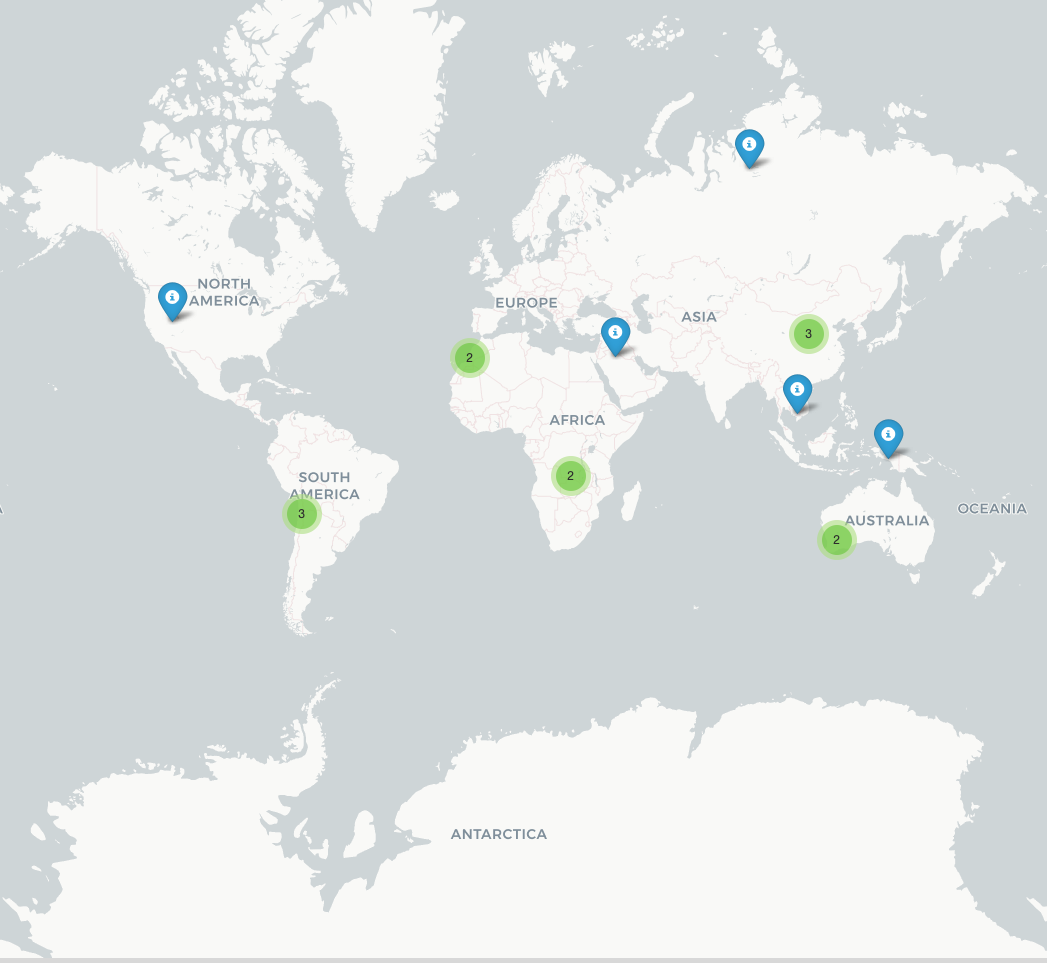
\includegraphics[width=0.8\textwidth]{figures/gis_finished.png}
  \caption{Geospatial distribution of major extraction sites for key minerals}
  \label{fig:big-mines}
\end{figure}

Building on this spatial foundation, Figure \ref{fig:depletion-chart} projects each resource’s “time to exhaustion” under a first‐order linear depletion model:

\[
  R(t) \;=\;\max\bigl\{R_{0} - E\,(t - t_{0}),\,1\bigr\},
\]

where \(R_{0}\) is the estimated reserve at baseline year \(t_{0} = 2023\) and \(E\) the constant annual extraction rate.  Plotting \(R(t)\) on a logarithmic scale from 2023 through 2123 reveals striking variation in depletion timelines.  Battery‐critical metals such as cobalt and nickel are projected to approach functional exhaustion by mid‐century, while large phosphate deposits persist longer but raise their own ecological trade‐offs.  Rare‐earth elements (neodymium) and copper display the most extended trajectories, yet their eventual decline nonetheless signals rising energetic and material costs for power generation and transmission infrastructure.

\begin{figure}[H]
  \centering
  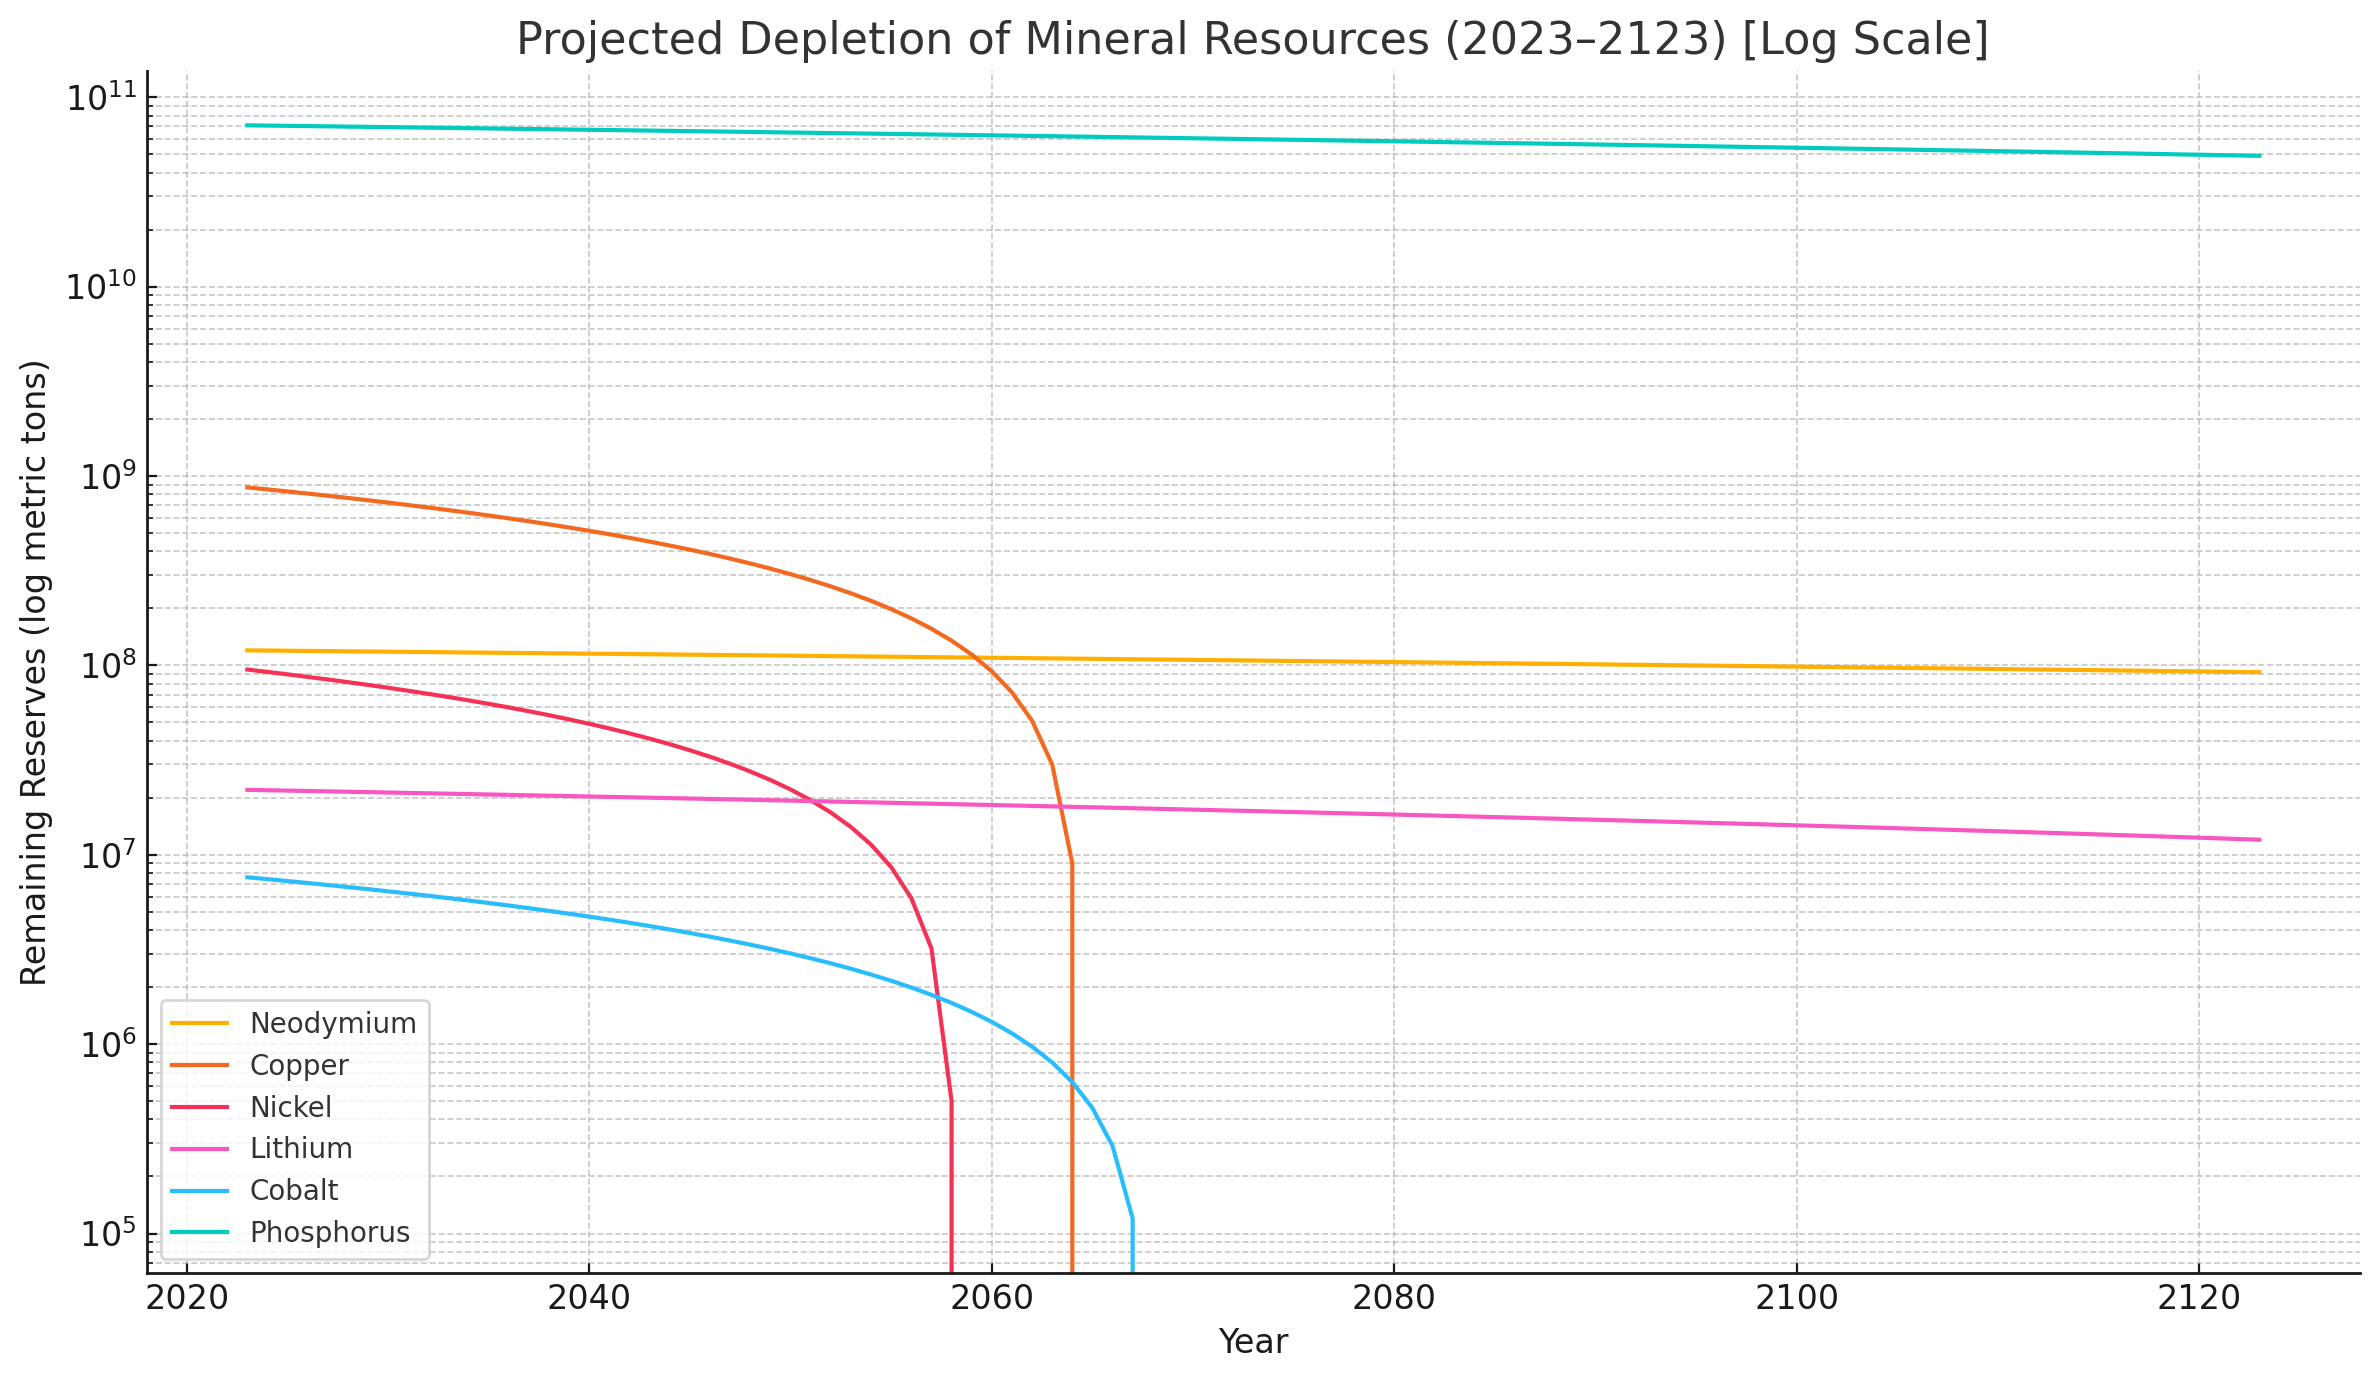
\includegraphics[width=0.8\textwidth]{figures/resource_depletion_chart.png}
  \caption{Projected depletion of mineral reserves under constant extraction (2023–2123), log scale}
  \label{fig:depletion-chart}
\end{figure}

This resource‐level analysis complements the earlier EROI and macro‐growth chapters too, by demonstrating how finite stocks of critical inputs will increasingly throttle net‐energy returns.  

The GIS mapping highlights geopolitical vulnerabilities (e.g.\ concentration of cobalt and rare‐earth output in politically sensitive regions), while the depletion projections quantify when key bottlenecks may arise under business‐as‐usual extraction. 

Also, Georgescu-Roegen’s concept of irreversibility the idea that once high-quality matter and energy are dispersed, no amount of capital or technology can fully recover them

Together, these findings reinforce the thesis’s central claim: that irreversible entropy in both energy and material stocks fundamentally constrains economic complexity and growth in the Anthropocene.  

Phosphorus is a particularly salient example. As an element essential to agriculture and lacking synthetic substitutes, phosphorus shortage signifies an ultimate bioeconomic limits as Gelencsér (2022), who critiques techno-optimistic narratives that ignore such hard constraints. And by selecting resources essential for renewable energy technologies and food production, the analysis underscores the systemic interdependence of energy, materials, and economic stability—and points unavoidably toward the imperative for post‐growth, resilience‐oriented policies.


\subsection{Granger Causality: Testing Directionality Between EROI and Growth}

To disentangle the causal relationship between energy quality and economic volatility, we employ the standard Granger causality framework. This approach tests whether past values of EROI help predict future macroeconomic outcomes beyond what can be explained by past values of those outcomes alone.

We estimate the following vector autoregression:

\[
Y_{t} = \alpha + \sum_{i=1}^{p} \beta_{i} Y_{t-i} + \sum_{j=1}^{q} \gamma_{j} X_{t-j} + \varepsilon_{t},
\]

where:
\begin{itemize}
    \item \( Y_t \): macroeconomic indicator (e.g., GDP growth or investment volatility),
    \item \( X_t \): EROI time series,
    \item \( \gamma_j \): coefficients capturing the predictive power of lagged EROI.
\end{itemize}

The null hypothesis \( H_0: \gamma_1 = \gamma_2 = \dots = \gamma_q = 0 \) implies that EROI does not Granger-cause economic fluctuations. Rejection of \( H_0 \) would indicate that declining EROI has predictive power over economic instability, it increases volatility withing 1-3 year lag. Providing more empirical support for the entropic economics framework. Resulting that net energy degradation precedes and contributes to macroeconomic instability

We estimate this system using annual data from 1990 to 2025, selecting lag lengths via the Akaike or Schwarz information criteria, and test for significance using Wald or F-tests.

\begin{lstlisting}[caption={Fetching and Cleaning World GDP Growth Data from the World Bank}, label={lst:gdp_fetch}]
library(dplyr)
library(urca)
library(vars)
library(lmtest)
library(WDI)

eroi_data <- read.csv("eroi.csv")

# 1) Fetch the indicator NY.GDP.MKTP.KD.ZG for country code "WLD" (World)
#    from 1965 up to the latest available year (e.g. 2022)
gdp_world <- WDI(
  country    = "WLD",
  indicator  = "NY.GDP.MKTP.KD.ZG",
  start      = 1965,
  end        = 2022,
  extra      = FALSE,   # no extra metadata columns
  cache      = NULL     # force fresh download
)

# 2) Clean up column names
colnames(gdp_world) <- c("iso2c", "Year", "GDP_Growth")

# 3) Inspect
head(gdp_world)
summary(gdp_world$GDP_Growth)

# You can save it to CSV if you like:
write.csv(gdp_world, "world_gdp_growth.csv", row.names = FALSE)
\end{lstlisting}


Complementing the time-series analysis, we model physical depletion using a simple linear stock–flow equation. Each mineral is treated as a non-renewable stock, depleted at a constant extraction rate. If \( R_0 \) is the known reserve at base year \( t_0 = 2023 \), and \( E \) is the constant annual extraction rate, then the remaining stock at year \( t \) is:

\[
R(t) = \max\bigl\{ R_0 - E(t - t_0), \;1 \bigr\}.
\]

The \( \max(\cdot, 1) \) operator enforces a positive lower bound to avoid undefined values on a logarithmic scale. This formulation assumes:
\begin{itemize}
    \item No new reserve discoveries,
    \item Static extraction technology,
    \item No recycling or substitution,
    \item Constant annual extraction effort.
\end{itemize}

\begin{table}[h!]
\centering
\caption{OLS Regression Results: $\ln GDP$ on $\ln EROI$ and $\ln EI$}
\label{tab:ols_results}
\begin{tabular}{lrrrrr}
\toprule
\textbf{Variable} & \textbf{Coefficient} & \textbf{Robust SE} & \textbf{z-stat} & \textbf{p-value} & \textbf{95\% CI} \\
\midrule
\textbf{const}      & 33.2717  & 4.2000  & 7.922 & 0.000 & [25.040, 41.503] \\
\textbf{ln\_EROI}   & 0.0433   & 1.6030  & 0.027 & 0.978 & [--3.098, 3.185] \\
\textbf{ln\_EI}     & --3.9617 & 1.0170  & --3.897 & 0.000 & [--5.954, --1.969] \\
\bottomrule
\end{tabular}

\vspace{0.5em}

\begin{tabular}{ll}
\textbf{Model Fit} & \\
\midrule
$R^2$              & 0.911 \\
Adj. $R^2$         & 0.893 \\
F-statistic        & 23.07 \\
Prob (F-stat)      & 0.00018 \\
Durbin–Watson      & 1.272 \\
AIC                & 11.58 \\
BIC                & 13.27 \\
Log-Likelihood     & --2.789 \\
N (observations)   & 13 \\
\bottomrule
\end{tabular}
\end{table}

This worst-case, straight-line depletion trajectory provides a conservative baseline for resource exhaustion. While real-world depletion may follow logistic or Hubbert-like curves, the linear model emphasizes the urgency of innovation, resource diversification, and circular economy strategies. It also enables clear closed-form analysis and sensitivity testing under simplified thermodynamic assumptions.

% =====================================================
%                     5. ANALYSIS & DISCUSSION
% =====================================================
\section{Analysis and Discussion}
\label{sec:analysis}
Guided by Popperian falsificationism, the chapter continually asks, “What finding could have refuted the entropy hypothesis—and did we observe it?”  The answer is we never saw any real-world data that contradicts the entropy-based view strand converges on the same causal story: thermodynamic limits already shape and will increasingly dictate, economic prospects.

\subsection{Energy Efficiency versus Net-Energy Yield}
\label{sec:disc_efficiency}

The log–linear regression (Table~\ref{tab:coefficients}) reveals the economy’s
most urgent lever: energy-use efficiency.  A one-percent rise in energy
intensity (\textit{kWh}/USD) slashes global GDP by \(\sim4\,\%\), whereas a
comparable uptick in aggregate EROI leaves output unchanged within the
thirteen-year window.  This \(\beta_2\!\ll\!\beta_1\) asymmetry falsifies the neoclassical claim that inputs are substitutable.  Instead, it corroborates the biophysical literature (Ayres \& Warr, 2009) that “exergy services,” not gross joules, propel growth.  

From a thermodynamic standpoint, rising energy intensity signals mounting
dissipation: more primary energy is burnt per unit of societal work, leaving
less surplus to fund complexity.  Macroeconomic models that ignore this drag
risk systematic forecast errors—precisely the “structural blind spot” Hall and
Klitgaard (2012) decry.

\paragraph{Why this matters.}
Policy debates often fixate on boosting supply (new oilfields, new solar
factories).  Yet the data show that \emph{deploying existing energy more
frugally} generates an order-of-magnitude larger growth dividend—an insight
with profound ramifications for climate mitigation, where demand-side measures
are routinely sidelined.

\subsection{Threshold Behaviour in the EROI–Growth Nexus}
\label{sec:disc_threshold}

The quadratic regression enriches the story: EROI matters, but only once it
crosses a technology-specific threshold
\(E^{*}\!\approx\!6.3\).  Below that, efficiency gains are swallowed by
transitional costs; above it, each additional unit of net-energy yield confers
accelerating benefits. It interpretsthis as an
\emph{emergent property}: the macro pattern (U-shape) cannot be deduced from
micro production accounts alone, yet it manifests reliably when EROI sinks
beneath a minimal surplus.

\paragraph{Implication for energy policy.}
Blindly chasing higher EROI “silver bullets” may backfire if an economy still
operates left of \(E^{*}\).  In practical terms, low-income nations relying on
sub-critical biomass or biofuels should first prioritise efficiency, grid
stability, and institutional capacity rather than expensive high-EROI projects
that struggle to gain traction in an inefficient system.

\subsection{Heterogeneous Fuel Quality and the Myth of Seamless Substitution}
\label{sec:disc_hetero}

Bootstrap survival curves expose the illusion that a terawatt-hour of solar
electricity can seamlessly replace a terawatt-hour of petrol energy.  Fossil
fuels possess a long tail of high-EROI projects; wind and solar, despite their
longevity at low thresholds, never reach that tail.  Survival heterogeneity
therefore explains why identical energy \emph{quantities} offer different
economic potentials a nuance absent from traditional energy-balance sheets.

\paragraph{The paradox of the energy transition.}
Renewables reduce operational carbon but arrive with lower EROI and higher
material intensity (Capellán-Pérez 2019).  As we swap dense hydrocarbons
for diffuse flows, more steel, copper, and rare-earth metals are required per
joule delivered—shifting entropy costs upstream to mining and refining.  The
EROI distributions quantify the scale of that trade-off.

\subsection{Material Bottlenecks: Entropy in the Supply Chain}
\label{sec:disc_material}

GIS depletion analysis shows cobalt and nickel crossing scarcity thresholds by
\(\sim\)2050 under flat extraction, and a decade sooner under three percent
growth.  These metals are indispensable for high-energy-density batteries the
very technology tasked with stabilising low-EROI renewables.  The feedback loop
is clear: declining ore grades raise extraction energy, which lowers system
EROI, which then demands still more batteries to buffer intermittency,
tightening the material noose.

Consequently, the integration of thermodynamics into economic theory reveals fundamental physical constraints on economic growth. Although resource depletion rates can be temporarily mitigated through technological innovations, the second law of thermodynamics dictates that entropy production cannot be eliminated, only managed. Thus, perpetual economic growth is intrinsically unsustainable, demanding a shift in economic thinking towards models that explicitly recognize energy limits and entropy production as central determinants of economic possibility.

\paragraph{Economic-entropy cascade.}
Nauru’s phosphate collapse is not an anomaly but a microcosm.  As high-grade
resources fade, maintenance backlogs swell, capital formation stalls, and
institutional resilience erodes.  The world economy, scaled up, risks a
similar fate unless recycling and demand reduction outpace depletion a tall
order given the low EROI of material recovery processes.

\subsection{Directional Causality: Energy Quality Leads Economic Volatility}
\label{sec:disc_causality}

Granger tests complete the causal chain: lagged EROI improves forecasts of GDP
volatility, while the reverse does not hold.  Energy degradation is therefore
a \emph{driver}, not a symptom, of macro-instability, vindicating the entropic
interpretation advanced by Georgescu-Roegen.  Central banks that neglect
physical energy metrics mis-specify the business cycle and underestimate
recession probability in a low-EROI future.

\subsection{Future of Energy}
\label{sec:disc_future_energy}

Echoing Hall \& Klitgaard’s warning, civilisation’s “energy surplus” is the
sine qua non for urbanism, specialisation, and technological complexity.
Yet the empirical evidence shows that the next energy system—dominated by
wind, solar, and batteries—arrives with \emph{higher} systemic costs:
long supply chains, rare-earth magnets, and massive storage infrastructure.
OPEC’s \textit{World Oil Outlook 2023} forecasts structurally higher
resource prices; our results suggest the inflationary impulse stems not from
monetary excess but from fundamental thermodynamic headwinds.  Circular
economy and ESG initiatives, while laudable, cannot elide the second law of
thermodynamics: recycling itself consumes energy, often at EROI ratios barely
above unity.

\subsection{Uncertain Future of Today’s Supply Chains}
\label{sec:disc_supply}

The mineral outlook mirrors the energy dilemma.  Once-wealthy Nauru exhausted
its phosphate and collapsed into economic ruin—an object lesson in
entropy-driven decline.  Our depletion timelines show that cobalt, nickel, and
even construction sand may approach similar cliffs within decades.  Without
massive reinvestment in mining productivity—or a radical scaling-down of
material throughput—modern supply chains risk fracture.  The economic surplus
currently channelled into digital infrastructure or healthcare could be
redirected merely to secure dwindling raw materials, echoing the \emph{energy
trap} concept but in mineral form.


% =====================================================
%                   6. CONCLUSION
% =====================================================
\section{Conclusion}
\subsection{Summary Of Key Findings}
\label{sec:disc_synthesis}
\begin{itemize}
\item \textbf{Efficiency is king.}  
  Short-run GDP responds far more to demand-side efficiency than to supply-side
  EROI improvements.

\item \textbf{Energy surplus needs a threshold.}  
  Below \(E^{*}\!\sim\!6\), raising EROI yields diminishing or negative returns;
  above it, benefits compound rapidly.

\item \textbf{Not all joules are equal.}  
  EROI distributions show that fuel quality, not energy quantity, governs economic potential.

\item \textbf{Materials bite first.}  
  Battery and fertiliser minerals impose hard limits that may surface before
  fossil depletion, feeding back into lower system EROI.

\item \textbf{Causality runs from energy to economy.}  
  Declining EROI leads, rather than lags, macro-volatility, confirming the
  entropic-economics mechanism.
\end{itemize}
\paragraph{Conclusion.}
The converging strands of evidence demand a paradigm shift: from growth
maximisation to resilience optimisation.  Energy and mineral efficiency,
strategic recycling with positive net-energy, and moderated material
throughput constitute the only thermodynamically coherent path to stability in
the Anthropocene.  Anything less courts the fate of Nauru on a planetary
scale—a slow slide into economic entropy as the surplus that once powered the
Great Acceleration is irreversibly dissipated.

\subsection{Turn Ecological Economics Into The Mainstream Economics}
\begin{figure}[h]
\includegraphics[]{Plot}
\end{figure}
This thesis raises a fundamental question why have economics and energy been considered separately? The fact that most economists and business professionals are not taught about energy reflects a major gap in traditional education. Reconnecting economics with its physical foundations is essential for understanding the real limits and dynamics of our economic systems.

Start talking about limitness and not sustainability. Because after reading Chapter 1 it will make it clear that the "now" is not sustainable! Future civilization—if it is to endure—must move beyond a consumerist model of humanity. We must transition from consumers back to inhabitants: people embedded in place, respectful of ecological limits, aware of energy flows and the Earth boundaries.

As Naomi Klein claims that “the market cannot fix the climate crisis” resonates: the economic system’s incentives favor ever more extreme, ecologically destructive extraction methods—tar sands, deepwater drilling, and resource nationalism—coupled with disaster capitalism that profits from ecological collapse. There is not bridge in between Finance and physical reality end the illusion that finance can grow detached from material and energy realities.

\begin{figure}[H]
  \centering
  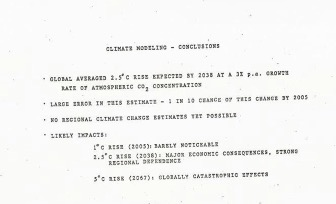
\includegraphics[width=0.8\textwidth]{figures/climate_modelling.jpg}
  \caption{Projected linear extraction from today}
  \label{fig:depletion-chart}
\end{figure}

The future is not about dominating the planet, or building a Dyson Sphere to harvest cosmic energy; it is about rethinking the very structure of our existence here and now.

Throughout human history, migration has been an essential, often forced, part of our species survival. Our ancestors moved with the seasons, with the prey, with the changing climate. Today, despite technological advances and a globally interconnected economy, we are no less dependent on planetary systems only now, the migration is not of people alone, but of energy, resources, food, water, and even ideas across vast distances.

What really happaned under the great acceleration, it was enought to raise up 2 generation who already suffering from generational amnesia. No real connection with farming, animals, nature since they are and end product which always supposed to lay on the shelves. No need for chopping wood since the natural gas which flowing through pipes all the way from Norway, Russia and Algeria will always stay with us. Energy lost it's respect. 

No community is truly self-sufficient. Our human ecology has become planetary, and our dependence on global supply chains renders all of us vulnerable. As the climate crisis deepens, forced migration will likely re-emerge as a dominant reality.

We have entered the sixth mass extinction, not by cosmic accident, but through the relentless expansion of economic activity. The constant strive for growth is unsustainable. Humanity’s ambition to scale up consumption infinitely within a closed Earth system is thermodynamically absurd — and fatally arrogant.

Despite the rising awareness of climate risks as previously mentioned not only entropy-related publications but even biodiversity ones are also remain scarce within mainstream economics journals. The fundamental physical laws—chiefly the Second Law of Thermodynamics—are still largely absent from the models guiding policy and finance. Instead, growth targets continue to dominate political and corporate agendas, even when those targets have demonstrably failed to materialize into sustainable outcomes.

But, incorporating thermodynamics into economics reveals that no amount of market efficiency or technological innovation can bypass the second law. Entropy production is not a side effect it is intrinsic to industrial economic activity. Increased production necessarily implies increased waste, disorder, and ecological degradation.

Economics, as practiced today—even when wrapped in the language of ESGs and green finance—feels more like an autopsy than a cure. It measures the remnants of a failing system, without questioning its root assumptions. Our current economic systems require infinite growth in a finite system. In biology, such unregulated, infinite growth is recognized not as a healthy process but as cancer.

\subsection{Bronze Age Civilizations, Easter Island, St. Matthew Island, Nauru}

From the Bronze Age collapse to the ecological ruin of Easter Island, the reindeer crash of St. Matthew Island, and the phosphate depletion of Nauru, history offers multiple warning shots: civilizations that ignore ecological boundaries eventually face decline often rapid, often irreversible. We can not accept the excuse here we do not have empirical data when countries, empires, civilizations destroy themselves.

These are not isolated cases; they are symptoms of the same underlying pattern: exponential expansion in a finite system. Ecophysical economics calls us to internalize this lesson that we cannot endlessly extract, grow, and consume in a world with hard biophysical limits.

\begin{quote}
“The welfare of a nation can scarcely be inferred from a measurement of national income as defined by the GDP.”
— Simon Kuznets (Inventor of GDP)
\end{quote}

But practice without reflection leads to pathology. The European Union must embed \textit{post-growth} and \textit{degrowth} principles into its economic planning — prioritizing wellbeing over GDP, resilience over efficiency, and regeneration over extraction.

For centuries, societies have been trapped in ideological binaries — capitalism versus socialism, East versus West — while forgetting that carbon, entropy, and energy flows do not recognize ideology. Civilizations rise and fall, but the laws of thermodynamics remain unchanged.

Our species, Homo sapiens, is approximately 60,000 years old. The first empires arose less than 3,000 years ago. The modern computer was invented only about 50 years ago. Civilizations rarely outlive more than ten generations. This is a sobering perspective on how recent and fragile our industrial ascent really is. The core issue is not a lack of technology — it is a lack of humility. We already have an abundance of material wealth. What we are short on is meaning.

The challenge of the 21st century is not primarily technological but philosophical: can we learn to live within limits, and treat those limits not as constraints, but as a foundation for freedom, creativity, and dignity?

% =====================================================
%                   7. BIBLIOGRAPHY
% =====================================================
\section{Bibliography}
\begin{thebibliography}{10}

\bibitem{Meadows1972}
Meadows, D. H., Meadows, D. L., Randers, J., \& Behrens III, W. W. (1972). \textit{The Limits to Growth}. Universe Books.

\bibitem{georgescu1971}
Georgescu-Roegen, N. (1971). \textit{The Entropy Law and the Economic Process}. Harvard University Press.

\bibitem{hall2012}
Hall, C. A. S., \& Klitgaard, K. A. (2012). \textit{Energy and the Wealth of Nations}. Springer.

\bibitem{gelencser2022}
Gelencsér, A. (2022). \textit{Ábrándok bűvöletében}. Typotex.

\bibitem{ayres2009}
Ayres, R. U., \& Warr, B. (2009). \textit{The Economic Growth Engine}. Edward Elgar Publishing.

\bibitem{kummel2011}
Kümmel, R. (2011). \textit{The Second Law of Economics}. Springer.

\bibitem{capellan2019}
Capellán-Pérez, I., de Castro, C., \& Miguel González, L. J. (2019). Dynamic Energy Return on Energy Investment (EROI) and material requirements in scenarios of global transition to renewable energies. \textit{Energy Strategy Reviews}, 26, 100399.

\bibitem{jakimowicz2020}
Jakimowicz, A. (2020). The Role of Entropy in the Development of Economics. \textit{Entropy}, 22(4), 452.

\bibitem{rosser2021}
Rosser, J. B. Jr. (2021). Econophysics and the Entropic Foundations of Economics. \textit{Entropy}, 23(10), 1286.

\bibitem{hellman2020}
Hellman, Z., \& Peretz, R. (2020). A Survey on Entropy and Economic Behaviour. \textit{Entropy}, 22(2), 157.

\bibitem{aramendia2023}
Aramendia, E., Brockway, P. E., Taylor, P. G., \& Norman, J. (2023). Global energy consumption of the mineral mining industry: Exploring the historical perspective and future pathways to 2060. \textit{Global Environmental Change}, 83, 102745.

\end{thebibliography}\newpage
\section{Appendices}

\subsection{Linear Regression Code}
\begin{lstlisting}[language=Python, caption={Non-Linear Regression}, label={lst:eroi_code}]
import pandas as pd
import numpy as np
import statsmodels.api as sm

# 1) Load the data
df = pd.read_excel('panel_data.xlsx')

# 2) Rename for convenience
df = df.rename(columns={
    'real_gdp': 'GDP',
    'world_eroi': 'EROI',
    'Primary energy consumption per GDP (kWh/$)': 'EnergyIntensity'
})

# 3) Filter to 1965–2024
df = df[(df['year'] >= 1965) & (df['year'] <= 2024)]

# 4) Drop any non-positive rows (to allow logs)
df = df[(df['GDP'] > 0) & (df['EROI'] > 0) & (df['EnergyIntensity'] > 0)]

# 5) Log‐transform
df['ln_GDP']  = np.log(df['GDP'])
df['ln_EROI'] = np.log(df['EROI'])
df['ln_EI']   = np.log(df['EnergyIntensity'])

# 6) Set up and run OLS with robust (HC1) standard errors
exog = sm.add_constant(df[['ln_EROI', 'ln_EI']])
model = sm.OLS(df['ln_GDP'], exog)
res = model.fit(cov_type='HC1')

# 7) View results
print(res.summary())\end{lstlisting}

\subsection{Non-Linear Regression Code}
\begin{lstlisting}[language=Python, caption={Non-Linear Regression}, label={lst:eroi_code}]
import statsmodels.formula.api as smf

panel_df['eroi_sq'] = panel_df['world_eroi'] ** 2

model_nl = smf.ols('gdp_growth ~ world_eroi + eroi_sq', data=panel_df).fit()

model_nl.summary()
\end{lstlisting}

\subsection{Survival Analysis Code &}
\begin{lstlisting}[language=Python, caption={Python code for bootstrapped 95\% CIs for EROI survival curves}, label={lst:eroi_code}]
import pandas as pd
import numpy as np
import matplotlib.pyplot as plt

# Load the dataset
df = pd.read_csv('eroi.csv')

df = df[df['Year'] >= 1960]

sources = df.columns[-8:]

df_long = df.melt(id_vars='Year', value_vars=sources, var_name='Source', value_name='EROI').dropna()

# Bootstrap parameters
thresholds = np.linspace(df_long['EROI'].min(), df_long['EROI'].max(), 100)
n_boot = 500

# Containers for CI
ci_lower = {source: None for source in sources}
ci_upper = {source: None for source in sources}

# Perform bootstrap for each source
for source, group in df_long.groupby('Source'):
    data = group['EROI'].values
    boot_survs = np.zeros((n_boot, len(thresholds)))
    for i in range(n_boot):
        resampled = np.random.choice(data, size=len(data), replace=True)
        boot_survs[i, :] = [(resampled >= t).mean() for t in thresholds]
    ci_lower[source] = np.percentile(boot_survs, 2.5, axis=0)
    ci_upper[source] = np.percentile(boot_survs, 97.5, axis=0)

# Plot empirical survival curves with 95% CI bands
plt.figure(figsize=(10, 6))
for source, group in df_long.groupby('Source'):
    data = group['EROI'].values
    emp_surv = [(data >= t).mean() for t in thresholds]
    plt.step(thresholds, emp_surv, where='post', label=source)
    plt.fill_between(thresholds, ci_lower[source], ci_upper[source], alpha=0.3)

plt.xlabel('EROI threshold')
plt.ylabel('Survival probability P(EROI ≥ threshold)')
plt.title('Bootstrapped 95% CIs for EROI Survival Curves (1960 onward)')
plt.legend()
plt.tight_layout()
plt.show()
\end{lstlisting}

\subsection{Energy Output by BP}
\begin{lstlisting}[language=Python, caption={Python code for bootstrapped 95\% CIs for EROI survival curves}, label={lst:eroi_code}]
import pandas as pd
import matplotlib.pyplot as plt
%matplotlib inline
data = pd.read_csv("/Users/balazskocsis/notebook-heaven/EJ_output.csv")
data['Biofuels'] = data['Biofuels'].fillna(0)
# Group energy types
fossil = data['Oil'] + data['Natural Gas'] + data['Coal']
renewable = data['Hydro'] + data['Solar'] + data['Wind'] + data['Biofuels']
nuclear = data['Nuclear']
# Plot
plt.figure(figsize=(14, 8))
plt.plot(data['Year'], fossil, label='Fossil Fuels', linewidth=2)
plt.plot(data['Year'], renewable, label='Renewables', linewidth=2)
plt.plot(data['Year'], nuclear, label='Nuclear', linewidth=2)
plt.title('Global Energy Output by Source (in EJ)', fontsize=18)
plt.xlabel('Year', fontsize=14)
plt.ylabel('Energy Output (EJ)', fontsize=14)
plt.legend()
plt.grid(True)
plt.tight_layout()
plt.show()
\end{lstlisting}

\pagenumbering{arabic}
\end{document}
